\documentclass[a4paper,10.5pt]{ctexart}
\usepackage[left=2.50cm, right=2.50cm, top=2.50cm, bottom=2.50cm]{geometry} %页边距
\usepackage{amsmath}
\usepackage{amssymb}
\usepackage{ctex}
\usepackage{braket}
\usepackage[table,xcdraw]{xcolor}
\usepackage[european]{circuitikz}
\usepackage{multirow}
\usepackage{float}
\usepackage{bm}         % 加粗方程字体
\usepackage{graphicx}
\usepackage{geometry}
\usepackage{helvet}
\usepackage[english]{babel}
\usepackage{booktabs}
\usepackage{indentfirst}
\geometry{left=2.0cm,right=2.0cm,top=2.0cm,bottom=2.0cm}
\usepackage{textcomp}
\usepackage{physics}
%\usepackage{algorithm}
%\usepackage{algorithmic}
\usepackage{longtable}
\usepackage{array}
\usepackage{xcolor}
\usepackage{algpseudocode}
\usepackage{epsfig}
\usepackage{arydshln}
\usepackage{textcomp}
%\usepackage[boxed]{algorithm2e}

\usepackage{algorithm,algpseudocode,float}
\usepackage{lipsum}
\makeatletter
\newenvironment{breakablealgorithm}
  {% \begin{breakablealgorithm}
   \begin{center}
     \refstepcounter{algorithm}% New algorithm
     \hrule height.8pt depth0pt \kern2pt% \@fs@pre for \@fs@ruled
     \renewcommand{\caption}[2][\relax]{% Make a new \caption
       {\raggedright\textbf{\ALG@name~\thealgorithm} ##2\par}%
       \ifx\relax##1\relax % #1 is \relax
         \addcontentsline{loa}{algorithm}{\protect\numberline{\thealgorithm}##2}%
       \else % #1 is not \relax
         \addcontentsline{loa}{algorithm}{\protect\numberline{\thealgorithm}##1}%
       \fi
       \kern2pt\hrule\kern2pt
       \renewcommand{\algorithmicensure}{\textbf{Output:}}
     }
  }{% \end{breakablealgorithm}
     \kern2pt\hrule\relax% \@fs@post for \@fs@ruled
   \end{center}
  }
\makeatother

\usepackage{listings} 
\usepackage{xcolor}

\lstset{
  language=Matlab,  %代码语言使用的是matlab
  frame=shadowbox, %把代码用带有阴影的框圈起来
  rulesepcolor=\color{white!},%代码块边框为淡青色
  keywordstyle=\color{blue!90}\bfseries, %代码关键字的颜色为蓝色,粗体
  commentstyle=\color{white!20!black!60!}\textit,    % 设置代码注释的颜色
  showstringspaces=false,%不显示代码字符串中间的空格标记
  numbers=left, % 显示行号
  numberstyle=\tiny,    % 行号字体
  stringstyle=\ttfamily, % 代码字符串的特殊格式
  breaklines=true, %对过长的代码自动换行
  extendedchars=false,  %解决代码跨页时,章节标题,页眉等汉字不显示的问题
   escapebegin=\begin{CJK*},escapeend=\end{CJK*},      % 代码中出现中文必须加上,否则报错
  texcl=true}



\newcommand{\PreserveBackslash}[1]{\let\temp=\\#1\let\\=\temp}
\newcolumntype{C}[1]{>{\PreserveBackslash\centering}p{#1}}
\newcolumntype{R}[1]{>{\PreserveBackslash\raggedleft}p{#1}}
\newcolumntype{L}[1]{>{\PreserveBackslash\raggedright}p{#1}}
\renewcommand{\algorithmicrequire}{ \textbf{Input:}}       
\renewcommand{\algorithmicensure}{ \textbf{Initialize:}} 
\renewcommand{\algorithmicreturn}{ \textbf{Output:}}    
\renewcommand{\figurename}{图}
\renewcommand\tablename{表} 
\makeatletter
\newcommand{\rmnum}[1]{\romannumeral #1}
\newcommand{\Rmnum}[1]{\expandafter\@slowromancap\romannumeral #1@}
\makeatother
%算法格式
\usepackage{fancyhdr}
\usepackage{subfigure}
\pagestyle{plain}

\lhead{}
\chead{}
\lfoot{}
\cfoot{}
\rfoot{}
\usepackage{hyperref} %bookmarks
\hypersetup{colorlinks, bookmarks, unicode} %unicode
\usepackage{multicol}

\begin{document}
	\begin{figure}[t]
		\parbox[b]{2cm}{
			
			}
		\parbox[b]{9cm}{
			\begin{center}
				\includegraphics[scale=0.8]{words.jpg}

				\small \textbf{ } 
			\end{center}
			}
	\end{figure}

	\begin{center}
		\quad \\
		\quad \\
		\vskip 3.5cm
		\heiti \zihao{2} 第三次上机作业	
	\end{center}


	\begin{center}
		\songti \fontsize{15}{15}
		\doublespacing
		
		\quad 

		\large191840004\hspace{0.6cm}蔡钟毓

	\end{center}
	\begin{center}
		\songti \fontsize{15}{15}
		\doublespacing
		
		\quad 

		\large2021年4月5日

	\end{center}

\clearpage

\date{}
%\sloppy
\bibliographystyle{unsrt}


%解决了什么问题、应用了什么方法、得到了什么结果;文字简练,突出新见解、新方法;最后书写(1000)
 %开头段:充分概括论文内容,两到三句话:简单交代题目背景;交代我们所做的事情(重要);这个问题的实际意义(可省)
\par %开头段:充分概括论文内容,两到三句话:简单交代题目背景;交代我们所做的事情(重要);这个问题的实际意义(可省)
从乙醇出发制备C$_4$烯烃是取代传统化石能源制备的有效路线,但由于转化过程中产物种类多、分布广导致乙醇转化率和C$_4$烯烃选择性低,人们设计了一种Co/SiO$_2$-HAP催化剂应用于催化乙醇偶合制备C$_4$烯烃。本文基于题给数据,建立统计回归模型,分析催化剂组合与温度对实验结果的影响,对探究C$_4$烯烃制备工艺条件具有一定参考价值。
\par \textbf{针对问题一:}%解决了什么问题、应用了什么方法(一定要结合题目说明)、得到了什么结果(计算数值答案/开放题简要答主要部分)
首先发现每组催化剂组合中乙醇转化率、C$_4$烯烃选择性与温度存在一定的关系,利用MATLAB的拟合工具箱Curve Fitting,用线性函数、指数函数、多项式函数和Fourier函数对数据进行拟合,分析结果为:乙醇转化率会随着反应温度单调上升,C$_4$烯烃选择性在大部分情况下随温度上升,在小部分催化剂组合下会出现峰值再回落的现象。接着对附件2数据的折线图初步分析,利用MATLAB的拟合工具箱Curve Fitting得到各个产物选择性关于时间的拟合函数$f_1(t)\sim f_5(t)$,分析结果为:乙醇转化率随时间推移降低,乙烯和乙醛选择性都随时间推移增加,其余产物变化较不规则。最后分析拟合效果:所有线性拟合函数的校正的$R^2$均值大于0.9,非线性拟合函数均方根误差接近0。
\par \textbf{针对问题二:}首先根据附件1数据,分析出乙醇转化率和C$_4$烯烃选择性的6个影响因素,基于控制变量原理,作出折线图进行定性分析。接着建立关于催化剂组合与温度和乙醇转化率与C$_4$烯烃选择性的多元线性回归模型,利用稳健标准误解决异方差问题,并得到方差膨胀因子VIF$_{max}$=1.39,因变量间相关性小。最终得到,对乙醇转化率:催化剂质量和温度起正向作用,乙醇浓度起负向作用,装料方式、Co负载量和装料比与其线性相关关系不显著;对C$_4$烯烃选择性:A类装料方式效果更好,乙醇浓度、催化剂质量和温度起正向作用,Co负载量起负向作用,装料比与其线性相关水平不显著。

%在其他变量给定的条件下,一定范围内,装料方式对二者影响不大,温度和催化剂质量起到显著的正向作用,乙醇转化率随乙醇浓度减小而显著升高,随装料比增加而升高,随Co负载量的增加出现先减后增的趋势;适当减小Co负载量对C$_4$烯烃选择性的增加有重要影响,乙醇浓度影响不明显,C$_4$烯烃选择性随着装料比增加出现先增后减趋势,在1:1时的值最大。

\par \textbf{针对问题三:}
%首先建立同问题二的六个变量与C$_4$烯烃收率之间的线性回归模型,模型拟合效果不佳,回归参数显著性水平低。
首先作出数据的柱状图进行定性分析,对自变量进行预处理并引入非线性自变量,建立影响C$_4$烯烃收率的非线性回归模型,运用稳健标准误解决异方差问题。分析结果如下:欲使C$_4$烯烃收率最高,应使用A类装料方式、Co/SiO$_2$质量200mg、与HAP的混料比1:1、Co负载量2wt$\%$、乙醇浓度0.9ml/min和反应温度400$^{\circ}$C;当要求温度低于350$^{\circ}$C时,应使用A类装料方式、Co/SiO$_2$质量200mg、与HAP的混料比1:1、Co负载量1wt$\%$和350$^{\circ}$C的反应温度。

\par \textbf{针对问题四:}采用“局部搜索”的思路设计5次新实验的参数:以 ${\rm C}_4$ 烯烃收率作为实验结果优劣的评判标准,将装料方式、Co/SiO$_2$质量、乙醇浓度和温度设定为问题三分析出的最优数值,仅对剩下2个在回归中不显著的变量进行微调。针对不同的实验情况设计两种方案:如果需要提前确定5次实验的全部参数,则给出5组实验参数使Co负载量和装料比分别在2wt$\%$和1附近浮动;如果可以在下一次实验参数确定前获得上一次实验结果,我们规定一套参数选取的规则来利用当前实验结果决定下一次实验的参数,同时保证收敛性和结果更优性。采用上述思路在已有的最优值附近进行搜索,有利于以较少的实验次数获得${\rm C}_4$烯烃收率的进一步改进。\\
~\\
\textbf{关键词:}C$_4$烯烃制备\quad 多元线性回归\quad 函数拟合\quad MATLAB\quad STATA
\clearpage

\section{问题重述}
%数学建模比赛论文是要我们解决一道给定的问题,所以正文部分一般应从问题重述开始,一般确定选题后就可以开始写这一部分了。
%这部分的内容是将原问题进行整理,将问题背景和题目分开陈述即可,所以基本没啥难度。
%本部分的目的是要吸引读者读下去,所以文字不可冗长,内容选择不要过于分散、琐碎,措辞要精练。
%注意:在写这部分的内容时,绝对不可照抄原题!(论文会查重)
%应为:在仔细理解了问题的基础上,用自己的语言重新将问题描述一遍。语言需要简明扼要,没有必要像原题一样面面俱到。
\par C$_4$烯烃作为重要的化工原料,广泛应用于化工产品和医药中间体的生产。在传统生产中,C$_4$烯烃的制备来源于化石能源,而随着化石能源的短缺以及其带来的日益严重的环境问题,人们渴望找到一种可持续的绿色新型能源用于制备C$_4$烯烃。其中,乙醇因具有污染小、来源广泛等一系列优点而被广泛研究并投入C$_4$烯烃的制备。如今,乙醇催化转化为C$_4$烯烃的研究已经获得优异成果,但由链增长反应机理可知,在制备过程中会出现产物分布广、种类杂、目标产物选择性低、应用价值差等问题。因此,为了提高C$_4$烯烃的选择性,人们通过设计合适的化学催化剂组合和温度,研究在相同实验条件下产物选择性的提高情况,以期探索乙醇催化偶合制备C$_4$烯烃的最佳工艺条件。\cite{article1}
\par 基于上述背景,我们将建立数学模型来解决以下问题:
\par \textbf{问题一}: 根据不同催化剂组合与温度下的结果,分析乙醇转化率、C$_4$烯烃的选择性与温度的关系;根据给定温度下某一次实验中各时间点的结果,分析各产物的占比和乙醇转化率与实验进行时间的关系。
\par \textbf{问题二}:根据收集的一系列实验结果,通过分析乙醇转化率和C$_4$烯烃选择性大小在不同催化剂组合与温度下的情况探究其中关系。
\par \textbf{问题三}:在相同的实验条件下,给出一个催化剂组合与温度设置方案,使C$_4$烯烃收率达到最高;当要求温度低于350度时,给出一个催化剂组合与温度设置方案以达到同样目的。
\par \textbf{问题四}:设计5个新的实验,以期获得更准确的C$_4$烯烃制备最优条件。

\section{问题分析}
\textbf{预备知识:}乙醇是生产制备C$_4$烯烃的原料,在制备的过程中,催化剂组合、温度、催化剂装料方式等可能会对C$_4$烯烃的选择性和C$_4$烯烃收率将产生影响。
其中,温度是指反应温度,选择性是指某个产物在所有产物中的占比,例如:在装料方式\Rmnum{1}下,250度时使用200mg 1wt\%Co/SiO$_2$- 200mg HAP-乙醇浓度1.68ml/min作为催化剂,乙烯选择性(\%)为1.17,是指在此条件下乙烯占所有产物的1.17\%。反应时间是指催化剂在乙醇氛围下的反应时间。
乙醇的转化率是指单位时间内乙醇的单程转化率,$C_4$烯烃收率的计算公式为:C$_4$烯烃收率=乙醇转化率$\times$ C$_4$ 烯烃的选择性。
\par 关于拟合工具箱的说明:Curve Fitting 是 MATLAB 内置的函数拟合工具箱,可以用于将给定的数据拟合成各种函数(如多项式函数、指数函数、Fourier 函数、正态分布函数、样条函数等),并进行不同拟合结果之间的比较。同时,工具箱还集成了输出评价指标、作图、生成代码等功能。

\subsection{问题一的分析}
对于C$_4$烯烃的制备,催化剂组合、温度、催化剂装料方式等将会对实验结果产生影响。本题控制催化剂不变,将温度作为自变量,研究乙醇转化率以及C$_4$烯烃的选择性与温度的关系。首先对附件1中的数据进行处理,仅保留催化剂、乙醇转化率、C$_4$烯烃的选择性、温度四个变量,控制催化剂不变,分别作出温度与乙醇转化率、温度与C$_4$烯烃的选择性的图像,观察图像后判断温度与乙醇转化率、温度与C$_4$烯烃的选择性的关系,并利用MATLAB进行拟合,得到两个函数关系。

再考虑附件2中的350度时给定的催化剂组合在一次实验不同时间的测试结果。由于时间序列的不均匀,无法采用时间序列分析,本题考虑以时间为自变量,乙醇转化率、乙烯选择性、C$_4$烯烃选择性、乙醛选择性、碳数为4-12脂肪醇选择性、甲基苯甲醛和甲基苯甲醇选择性以及其他乙醇转化率为因变量,进行函数的拟合,得到乙醇转化率关于时间的函数,以及各个产物选择性与时间的关系。在研究各个产物与时间的关系时,可能出现某一个产物选择性难以拟合的情况,此时考虑产物选择性之和为100\%,通过100\%减去其余产物的选择性质和,亦可得到该产物的选择性与之间的关系函数。

\subsection{问题二的分析}
先对附件1中数据进行描述统计,了解数据大致的分布情况,得到下图:
\begin{figure}[h]
\centering
\begin{minipage}[t]{0.48\textwidth}
\centering
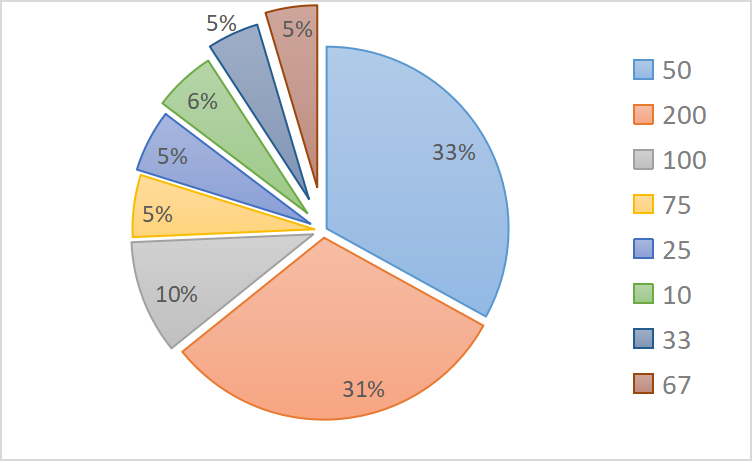
\includegraphics[width=9cm]{CoSiO2质量.png}
\caption{Co/SiO$_2$质量的饼状图}
\end{minipage}
\begin{minipage}[t]{0.48\textwidth}
\centering
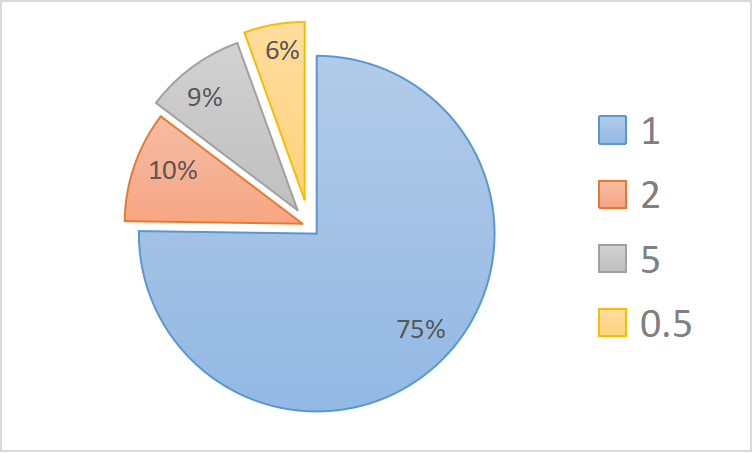
\includegraphics[width=9cm]{Co负载量.png}
\caption{Co负载量的饼状图}
\end{minipage}
\end{figure}


\begin{figure}[h]
\centering
\begin{minipage}[t]{0.48\textwidth}
\centering
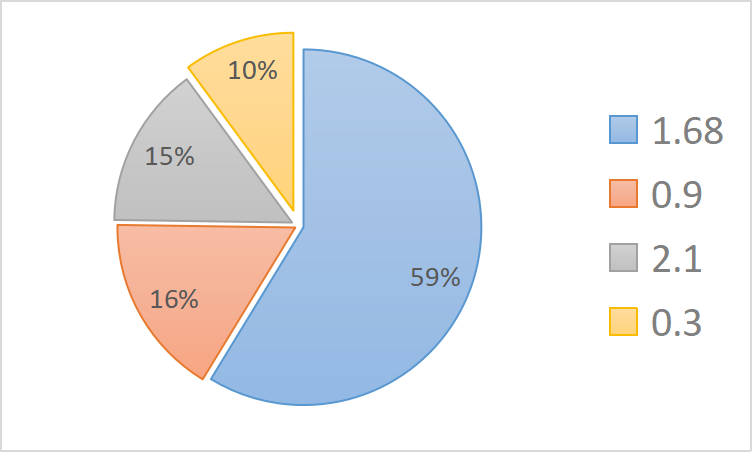
\includegraphics[width=9cm]{乙醇浓度.png}
\caption{乙醇浓度的饼状图}
\end{minipage}
\begin{minipage}[t]{0.48\textwidth}
\centering
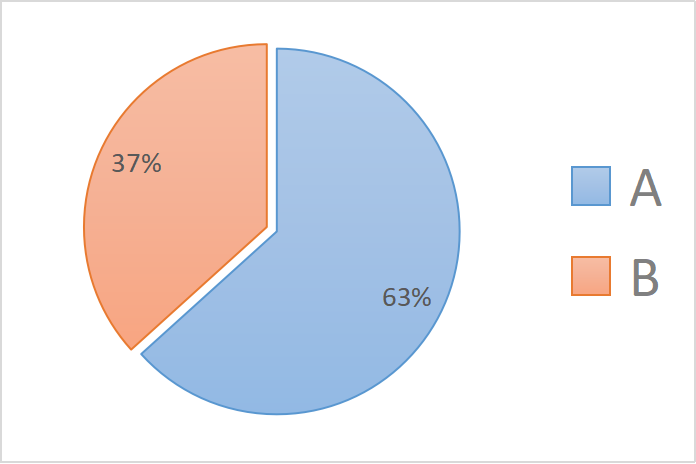
\includegraphics[width=9cm]{装料方式.png}
\caption{装料方式的饼状图}
\end{minipage}
\end{figure}
问题二考虑乙醇转化率和C$_4$烯烃选择性大小与不同催化剂以及温度的关系,将催化剂及其装料方式转化成五个变量,由这五个变量可以唯一确定一种催化剂与装料方式,并且五个变量之间互不相关,将温度也作为自变量,则有六个自变量共同决定乙醇转化率和C$_4$烯烃的选择性。首先利用控制变量,画出折线图,观察乙醇转化率以及C$_4$烯烃的选择性大小与催化剂的各个要素以及温度之间是否存在线性关系,以及是否呈正关系或负关系;然后,可以利用多元线性回归对各自变量对乙醇转化率和C$_4$烯烃的选择性大小的影响进行具体的分析;得到回归方程后,检验回归关系与参数的显著性,再利用怀特检验考察异方差,若扰动项存在异方差,则需要对异方差进行处理。

\subsection{问题三的分析}
\input{问题三分析.txt}

\subsection{问题四的分析}
\par 问题四研究增加的 5 次实验如何选择催化剂组合和温度的问题。由于我们的总目标是探索如何在化学反应中更高效地制备 ${\rm C}_4$ 烯烃,因此再增加 5 次实验的目标也应当是获得更高的 ${\rm C}_4$ 烯烃收率。在上一个问题中研究了 ${\rm C}_4$ 烯烃收率与催化剂组合、温度的关系,然而已有的实验数据总共是 109 次,远远大于增加的 5 次,所以如果把新的 5 次实验连同已有的实验数据,再次放到上一个问题的模型中进行求解,得到的新解与上一个问题的结果相比,产生的变化很可能是微小的。
\par 因而,相比于补全已有的实验数据,新增加的 5 次实验的作用更可能是在已有的最优催化剂组合和温度附近进行局部搜索。换言之,在已有的最优数值的附近进行微调,收益可能远远高于填补原有实验数据的空缺。新的 5 次实验的参数也将按照“最优解附近局部搜索”的思路进行设计。
\section{模型假设}

\par 1.假设观测的数据的误差可忽略不计;

2.假设每次实验中除了催化剂组合和温度,其余变量均相同;

3.假设没有环境因素的影响:在相同大气压、空气湿度等情况下下进行实验。
\section{符号说明}
%本部分是对模型中使用的重要变量进行说明,一般排版时要放到一张表格中。
%注意:第一:不需要把所有变量都放到这个表里面,模型中用到的临时变量可以不放。第二:下文中首次出现这些变量时也要进行解释,不然会降低文章的可读性。
\begin{table}[h]
\centering
\begin{tabular}{C{2cm}C{12cm}C{2cm}}
\toprule[2pt]
\textbf {符号}&\textbf {定义}&\textbf {单位}\\\midrule[1pt]
T& 反应温度  &$^{\circ}$C \\
t& 反应时间  &min \\
$y_1$& 乙醇转化率 & $\%$\\
$y_2$& C$_4$烯烃选择性 & $\%$\\
$x_1$ &装料方式& $\backslash$\\
$x_2$&Co负载量 &wt$\%$\\
$x_3$& Co/SiO$_2$质量& mg\\
$x_4$ & 装料比(HAP质量:Co/SiO_2质量) & $\backslash$\\
$x_5$ & 乙醇浓度& ml/min \\
$z$ & C_4烯烃收率($y_1 \times y_2$)& \textpertenthousand  \\
\bottomrule[2pt]
    \end{tabular}%
  \label{tab:addlabel}%
\end{table}%

注:未列出符号及重复符号以出现位置为准
\section{模型的建立与求解}
\subsection{问题一模型的建立与求解}
\subsubsection{第一问模型的建立与求解}
\input{模型求解一.txt}
\subsubsection{第二问模型的建立与求解}

考虑350度时给定的催化剂组合在一次实验不同时间的测试结果,并对结果进行分析。

利用MATLAB做出乙醇转化率关于时间的变化曲线以及各种生成物关于时间的变化折线,得到下图:
\begin{figure}[h]
\centering
\begin{minipage}[t]{0.45\textwidth}
\centering
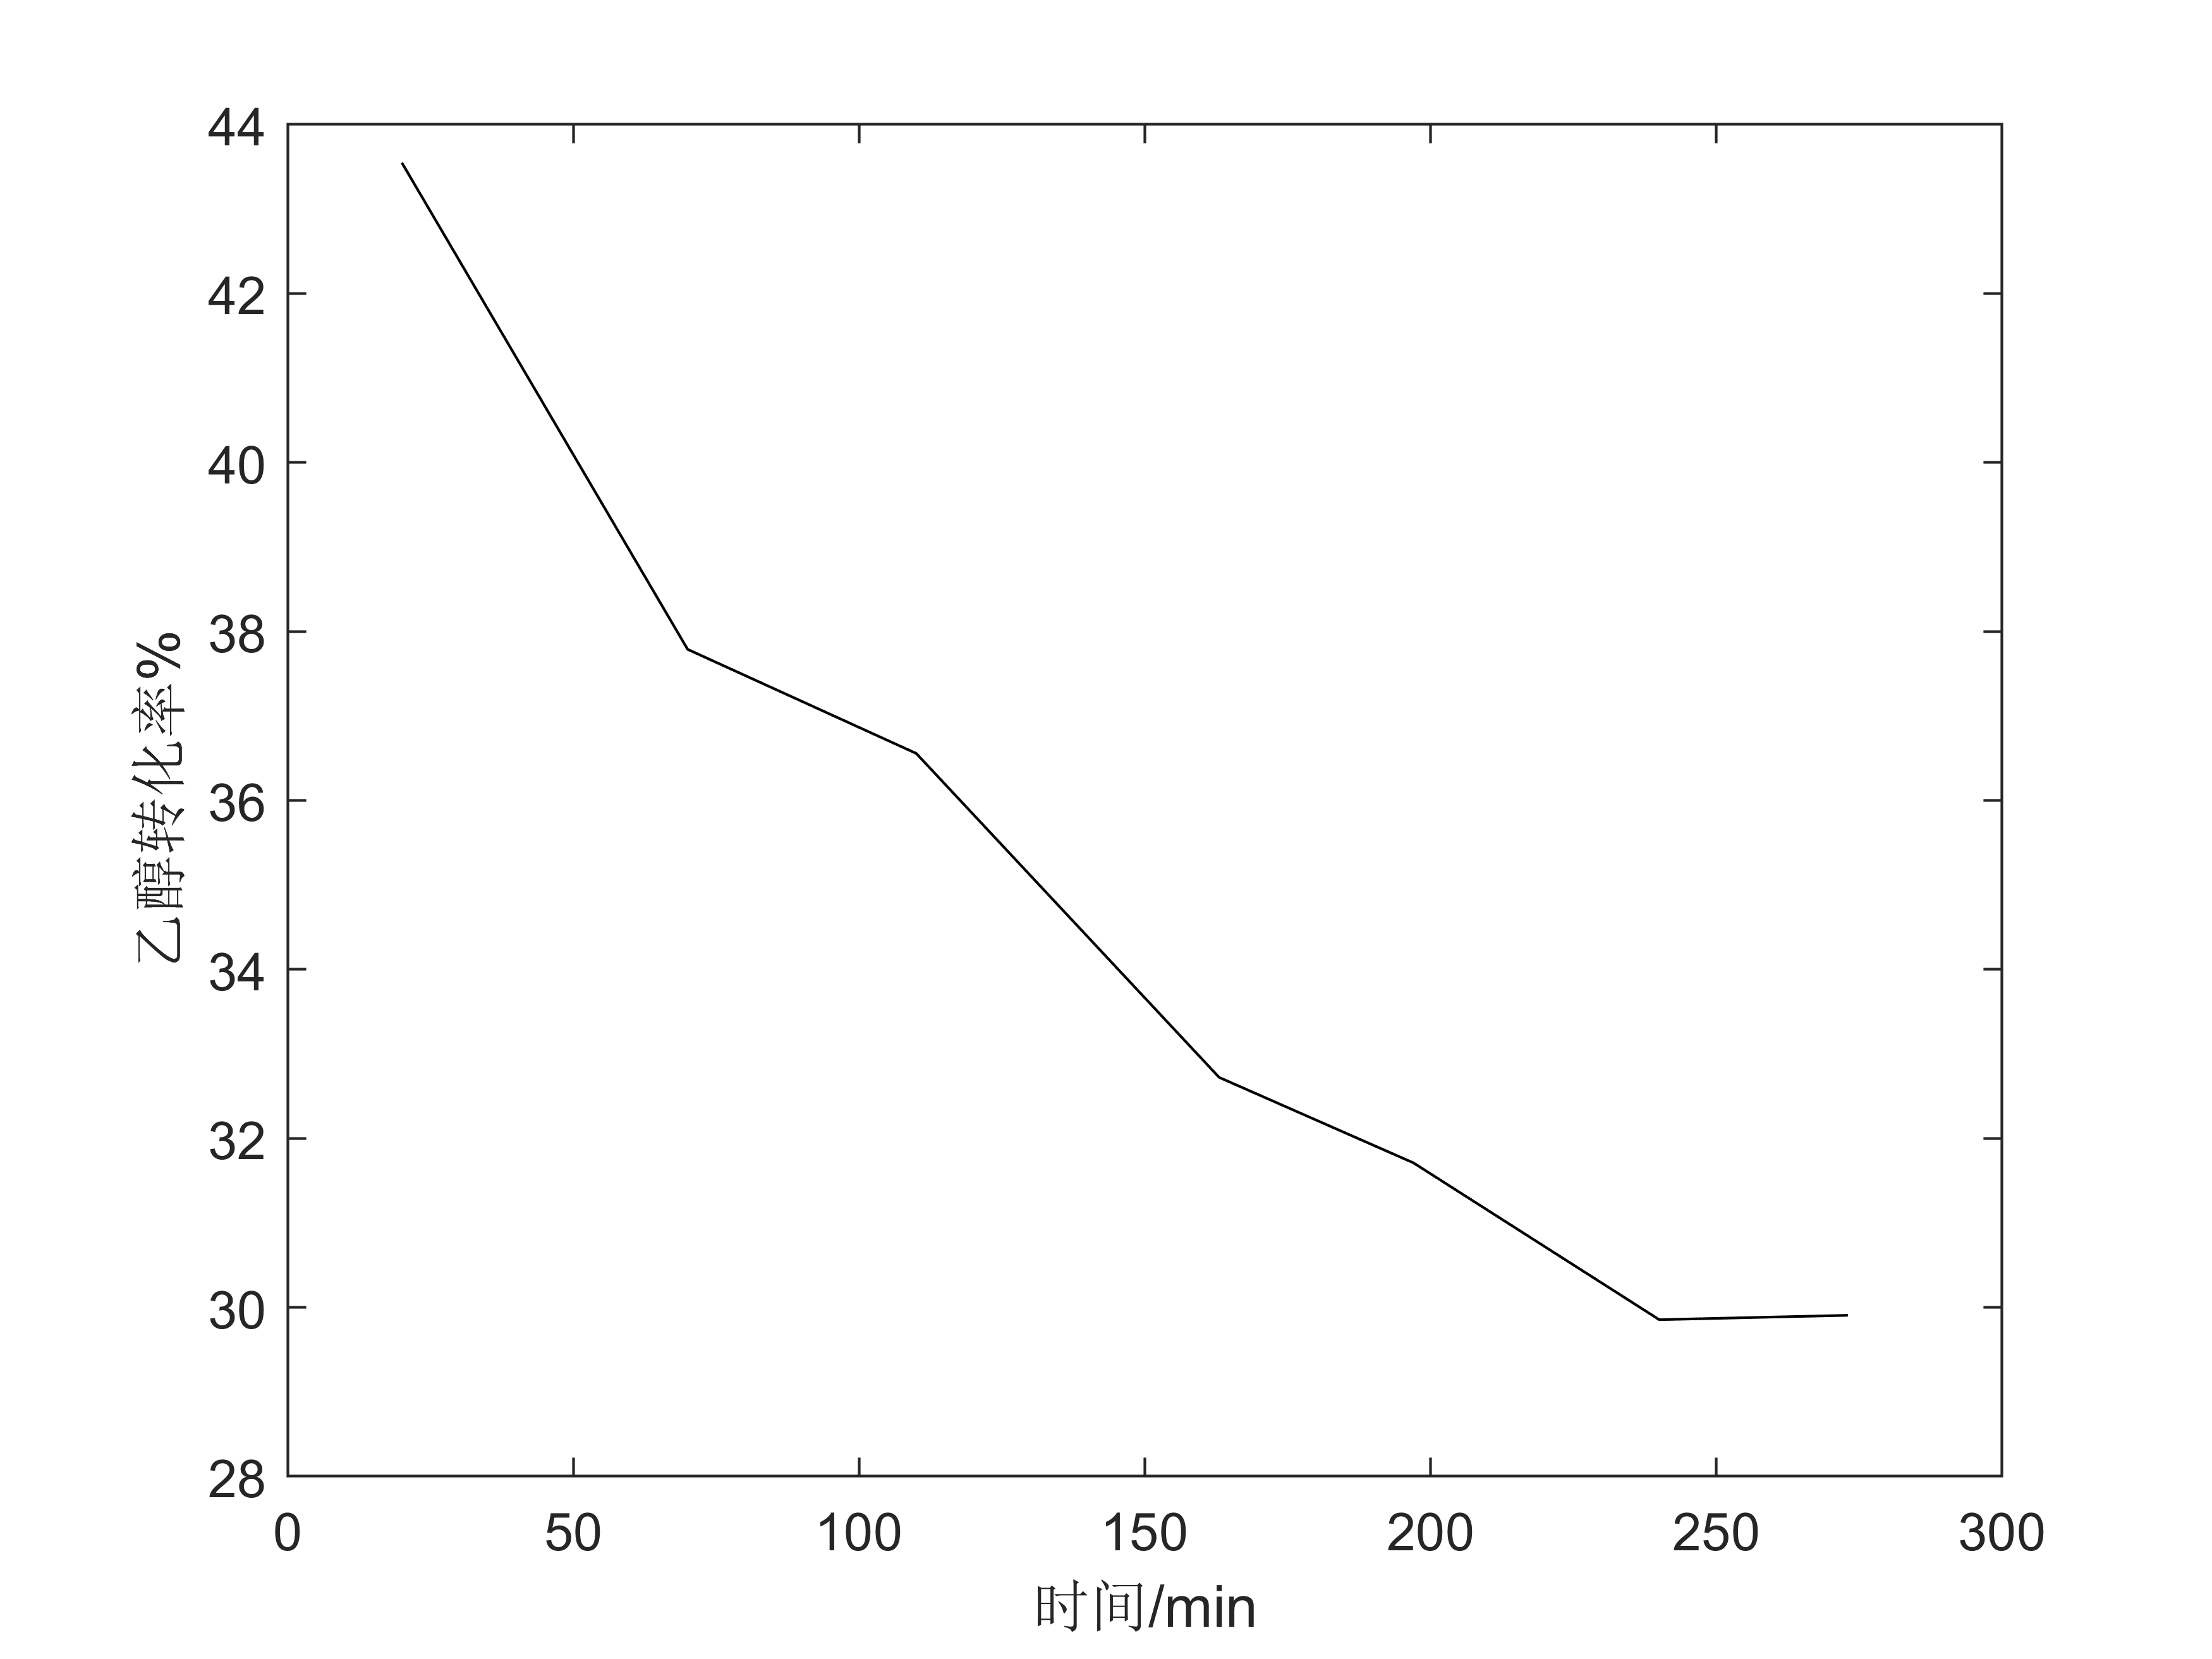
\includegraphics[width=7cm]{乙醇转化率.png}
\caption{乙醇转化率关于t的折线}
\end{minipage}
\begin{minipage}[t]{0.54\textwidth}
\centering
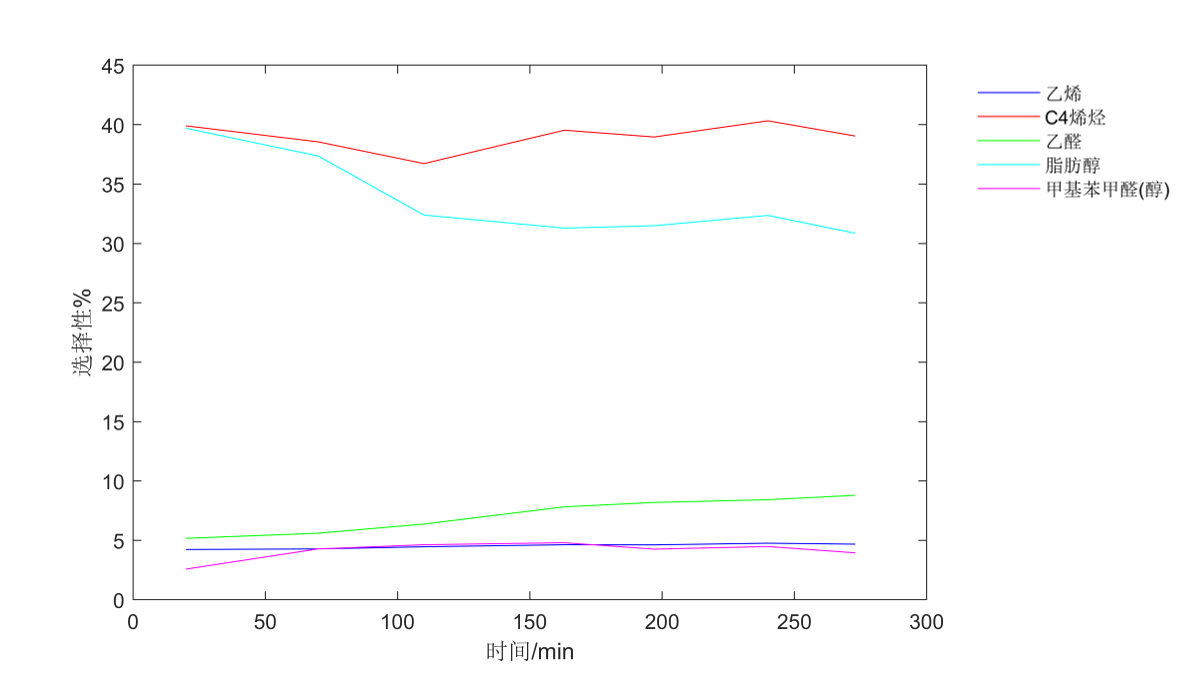
\includegraphics[width=9cm]{选择性与时间.png}
\caption{各产物选择性关于t的折线}
\end{minipage}
\end{figure}

观察图11可以发现,乙醇转化率与时间有明显的关系,乙醇转化率随时间的增加而逐渐减小,乙醇转换速率放缓;观察图12可以得到,C$_4$烯烃的选择性与脂肪醇的选择性明显高于其余三种产物,可以猜测C$_4$烯烃与脂肪醇是该实验的主要产物,观察随时间增加各产物的变化,发现乙醛的选择性随时间增加而增加,脂肪醇的选择性随时间增加而减少,而C$_4$烯烃与乙烯、甲基苯甲醛(醇)的选择性与时间并没有明显的线性关系。下面考虑利用MATLAB分别拟合各个产物选择性关于时间的函数,从而进一步分析时间对于实验结果的影响。

对于不同产物选择性与时间的变化关系,使用MATLAB拟合工具箱进行拟合,拟合函数的选取方式与 5.1.1 中相同。考虑到所有产物的选择性之和为100\%,故而C$_4$烯烃选择性关于时间的关系受到其它产物的影响,除乙烯选择性、C$_4$烯烃选择性、乙醛选择性、碳数为4-12脂肪醇选择性、甲基苯甲醛和甲基苯甲醇选择性以外,还有其它产物,受到此类产物的影响,C$_4$烯烃选择性难以获得较好的函数拟合。在多次实验之后,得到均方误差最小的拟合函数图像如下:
\begin{figure}[h]
\centering
\begin{minipage}[t]{0.48\textwidth}
\centering
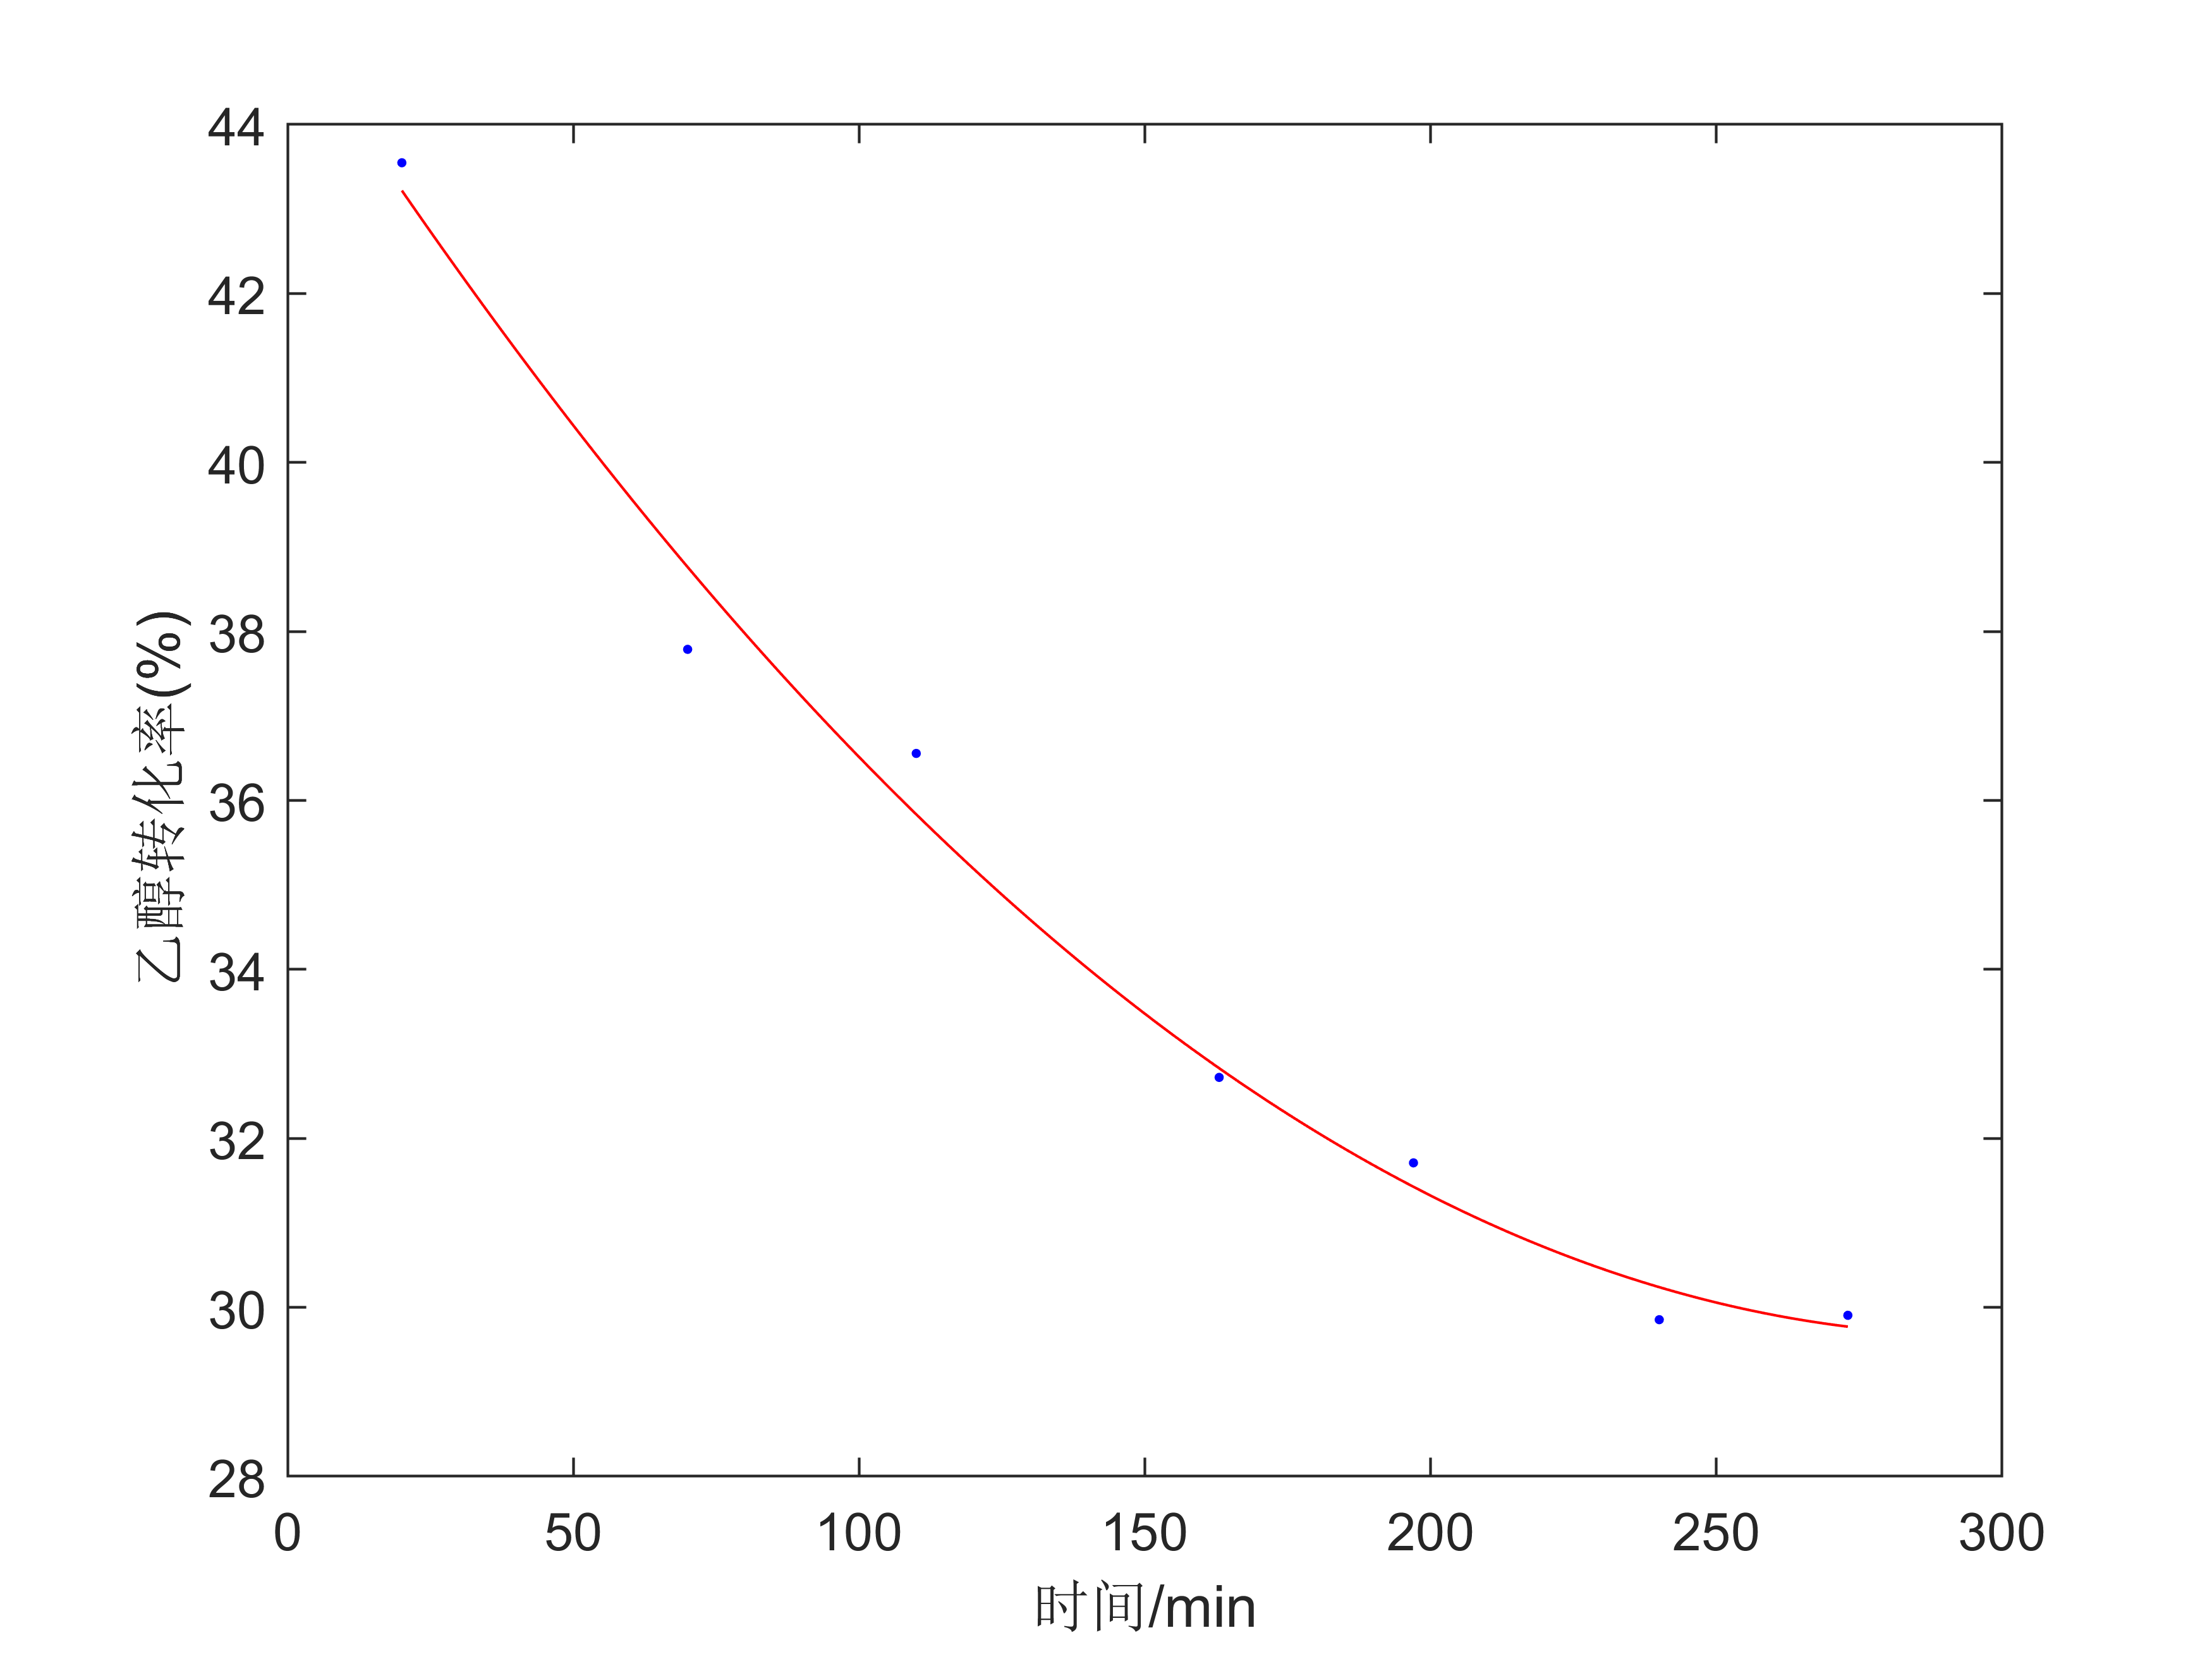
\includegraphics[width=6cm]{time-乙醇.png}
\caption{乙醇转化率关于t的拟合函数$f_1(t)$}
\end{minipage}
\begin{minipage}[t]{0.48\textwidth}
\centering
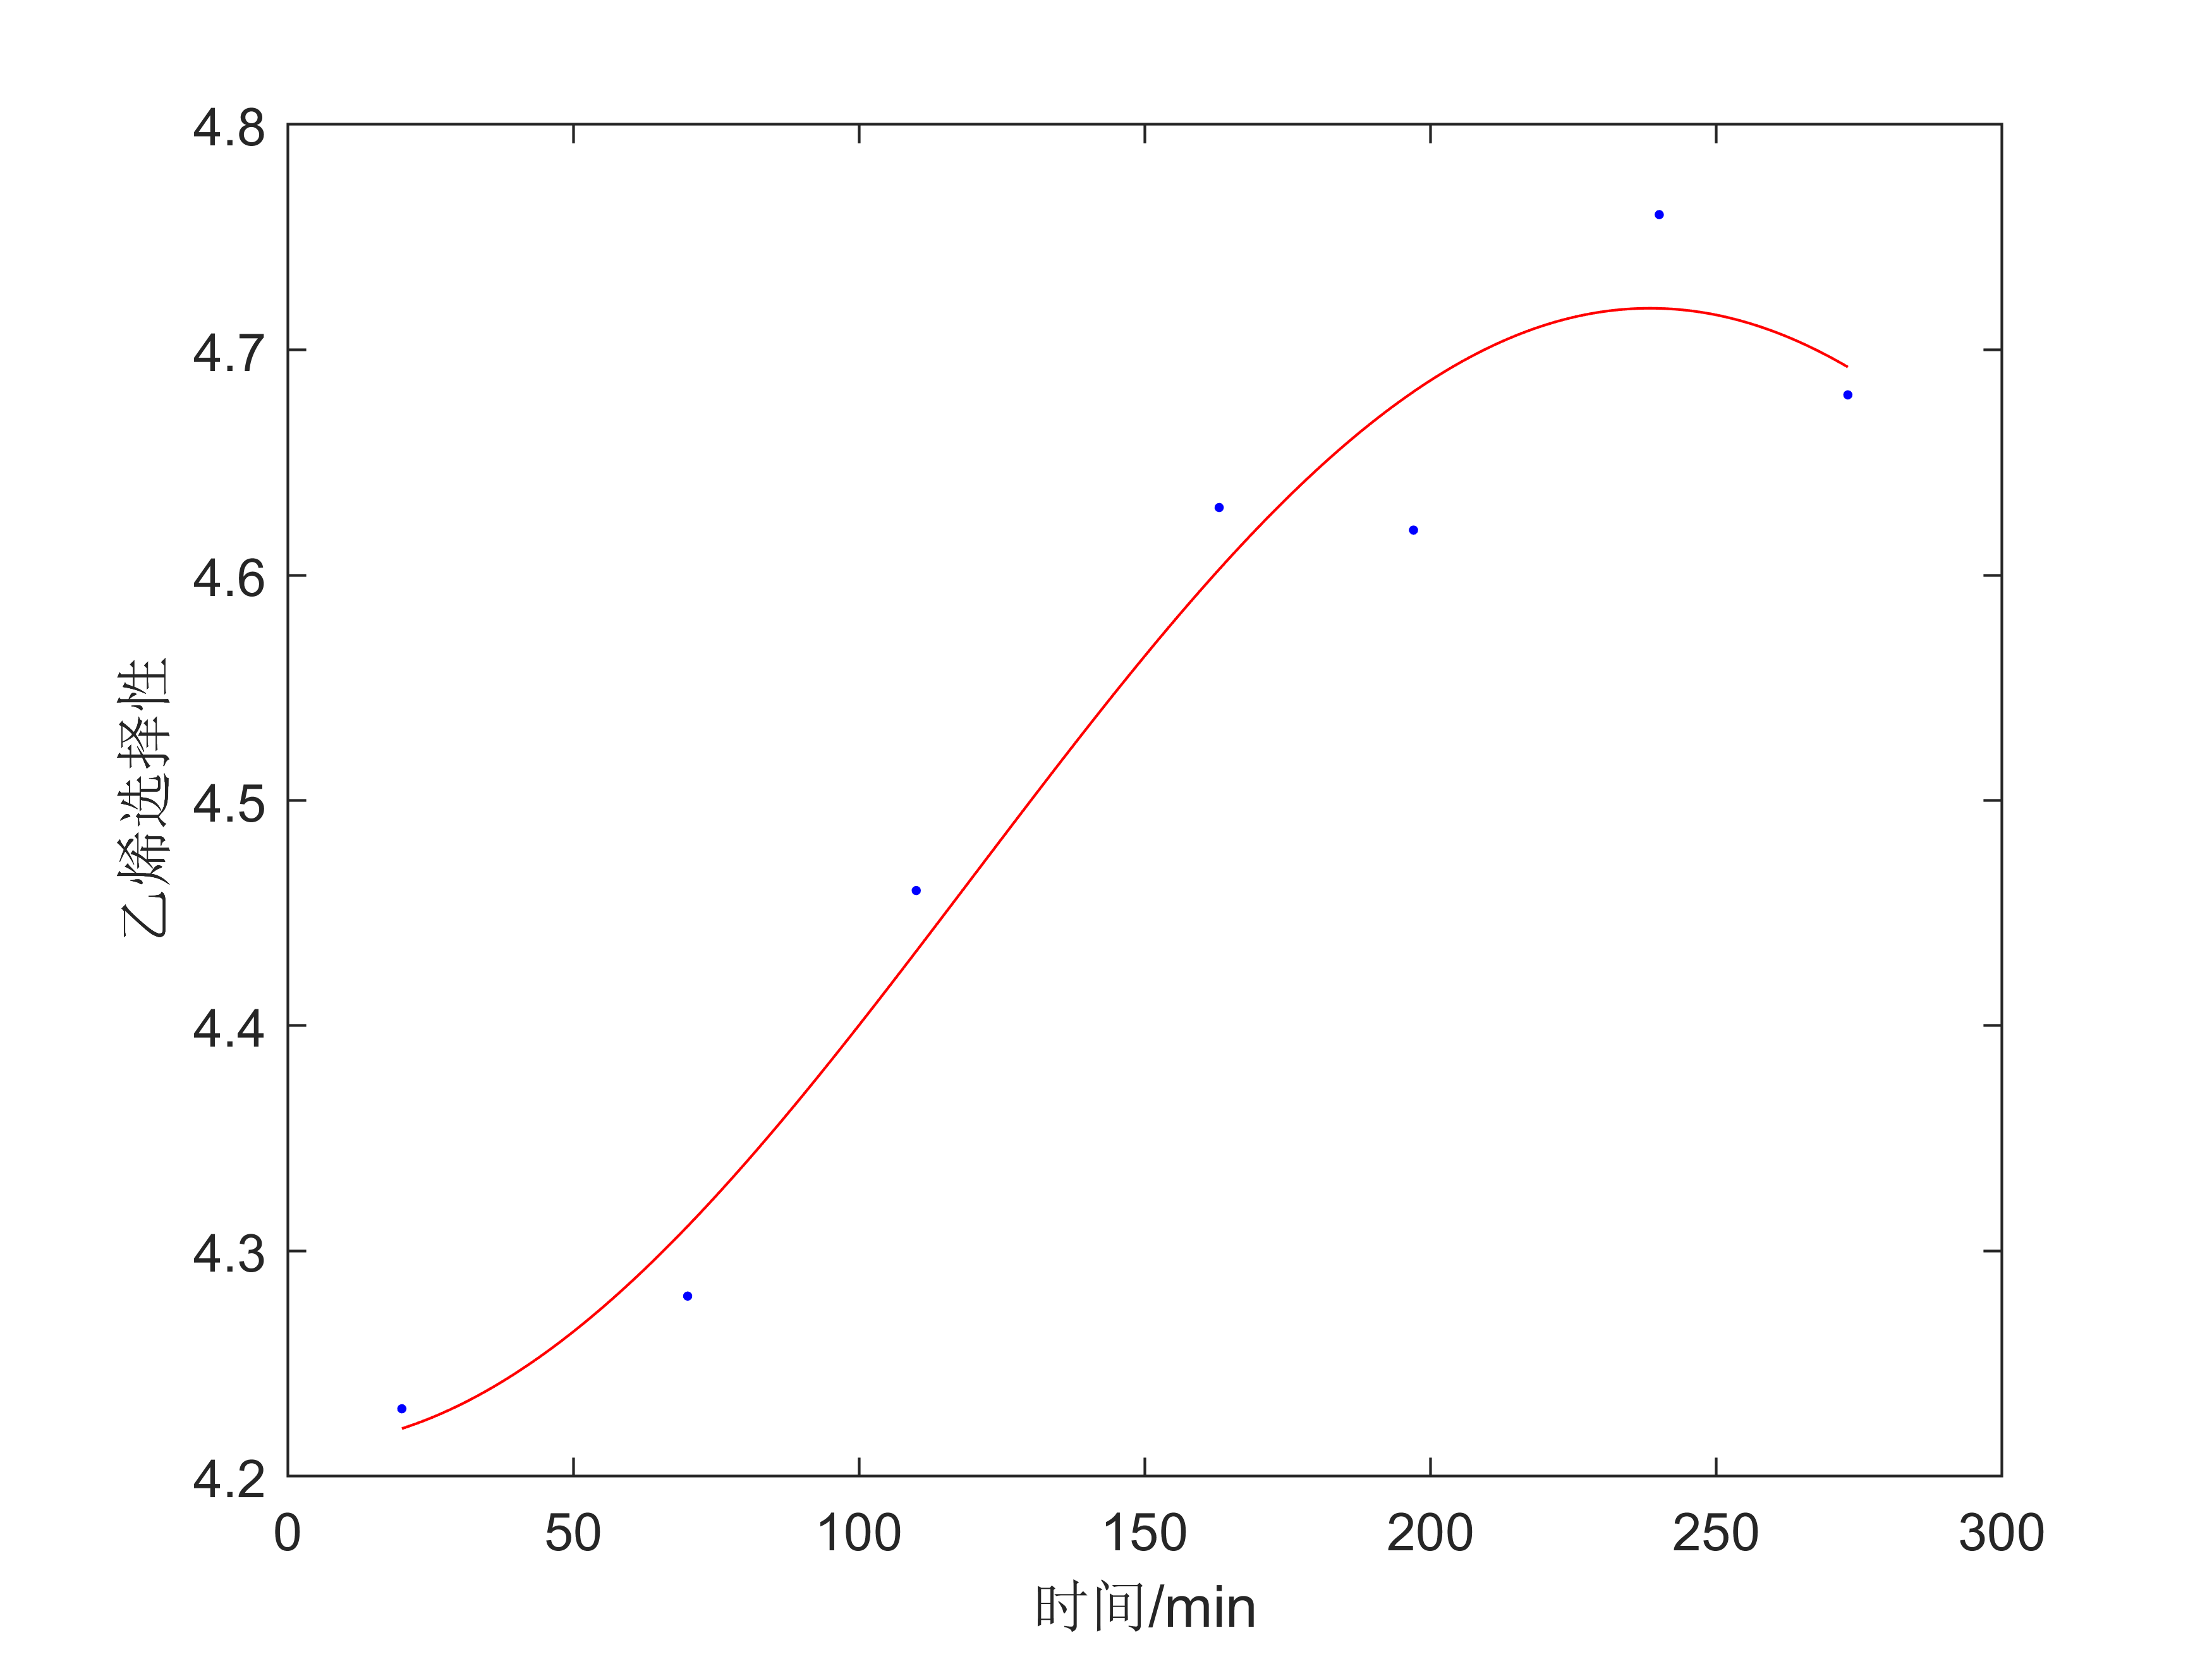
\includegraphics[width=6cm]{time-乙烯.png}
\caption{乙烯选择性关于t的拟合函数$f_2(t)$}
\end{minipage}
\end{figure}

\begin{figure}[h]
\centering
\begin{minipage}[t]{0.48\textwidth}
\centering
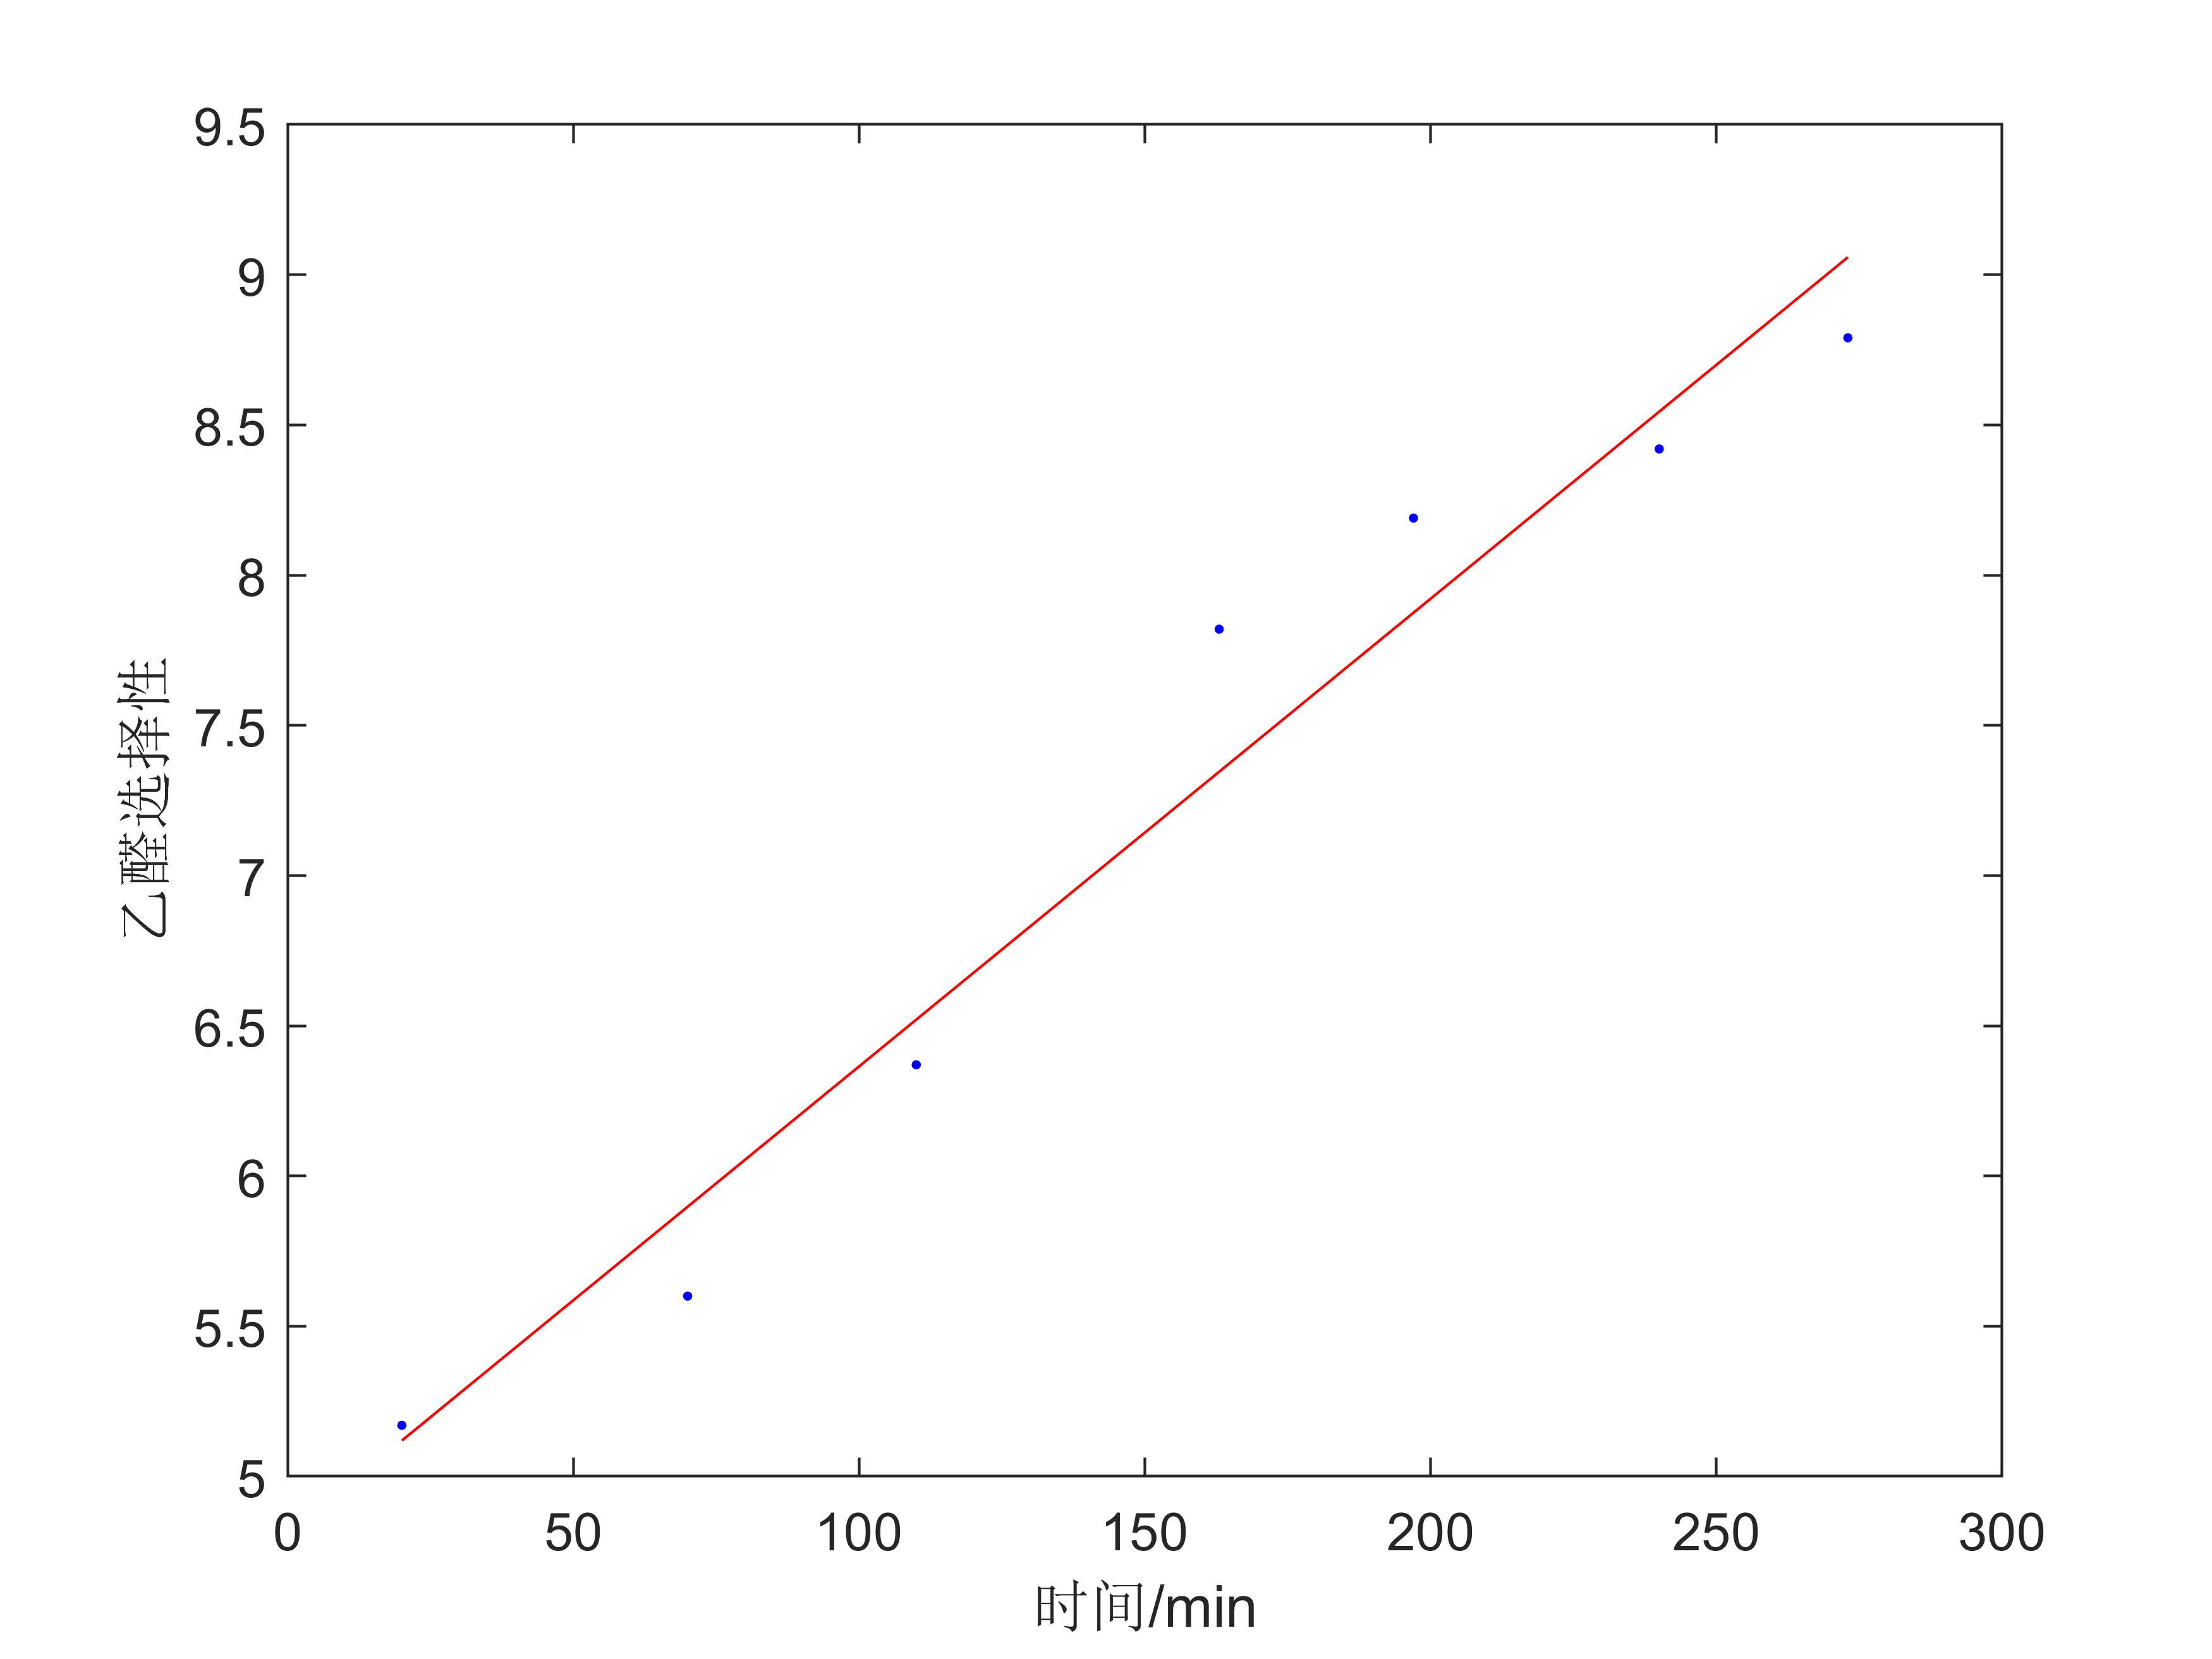
\includegraphics[width=6cm]{time-乙醛.png}
\caption{乙醛选择性关于t的拟合函数$f_3(t)$}
\end{minipage}
\begin{minipage}[t]{0.48\textwidth}
\centering
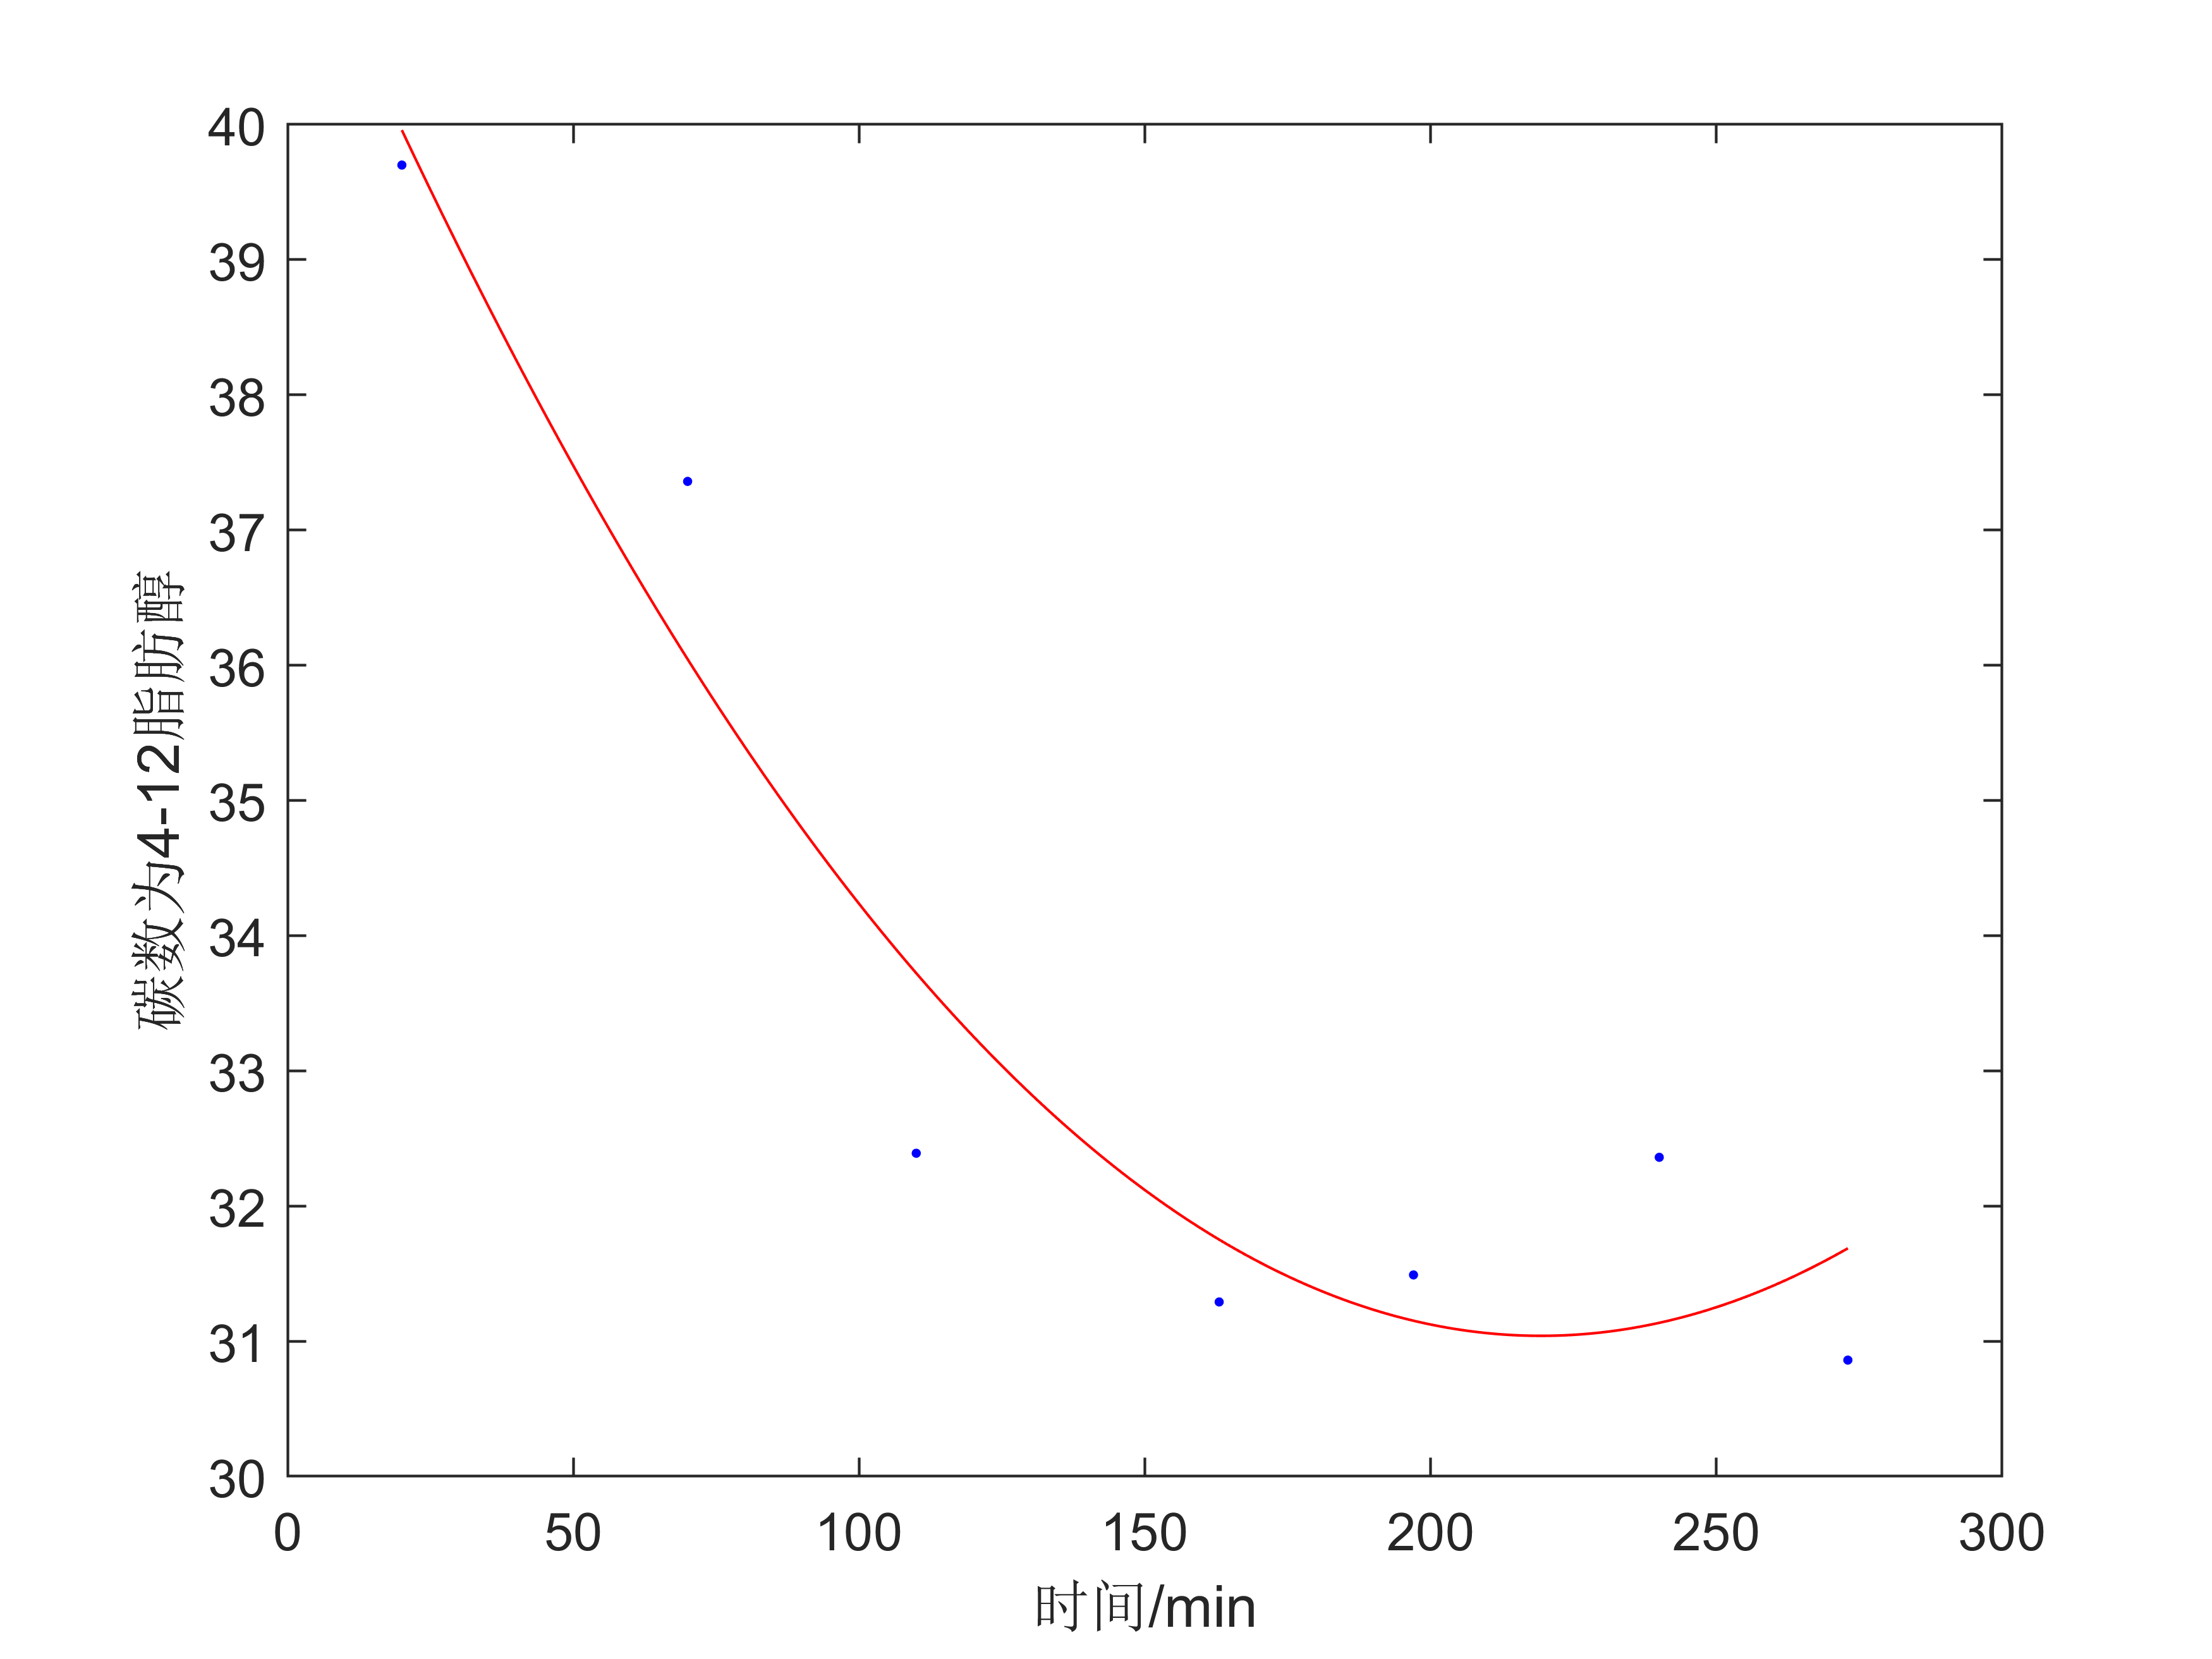
\includegraphics[width=6cm]{time-脂肪醇.png}
\caption{\certering 脂肪醇选择性关于t的\\拟合函数$f_4(t)$}
\end{minipage}
\end{figure}
\vspace*{130pt}
函数关系式分别为:


\begin{equation}
\begin{aligned}
\nonumber
f_1(t)&=0.0001772t^2-0.1051t+45.25 \\
f_2(t)&=4.466-0.2524\cos(0.01325t)-0.004488\sin(0.01325t)\\
f_3(t)&=0.01557t+4.808\\
f_4(t)&=0.0002245t^2-0.09848t+41.84\\
f_5(t)&=4.753\times10^{-7}t^3-0.0002985t^2+0.05497t+1.631\\

\end{aligned}
\end{equation}

考察上述拟合函数的拟合优度,发现对于线性函数关系,拟合优度$R^2> 0.91$(具体回归评价指标见模型的分析与检验部分),故而可以利用上述函数作为各产物选择性关于时间的近似关系。观察图像以及函数关系式可以得到:乙醇转化率随时间的增加而降低,而乙烯选择性以及乙醛选择性都随时间增加有明显的增加;脂肪醇的选择性随时间增加而先降低,而到230min左右,脂肪醇的选择性又随时间的增加而产生一定的上升趋势;甲基苯甲醛(醇)的选择性在130min之前随时间的增加有显著的增长,而130min后增长放缓甚至开始下降;C$_4$烯烃的选择性在100min之前随时间增加有明显的增加,而100min之后增长放缓,并于150min后下降。




\subsection{问题二模型的建立与求解}

\subsubsection{模型的建立}
\par \textbf{step 1} 对乙醇转化率与C$_4$烯烃选择性的影响因素进行分析:
\par 从附件1给出的性能数据中可以看出,在不同的催化剂组合和温度下,乙醇的转化率和各产物的选择性不同。催化剂组合中的变量包含:Co负载量、Co/SiO$_2$和HAP的装料比、乙醇浓度和装料方式。同时,根据对附件1中数据的观察,在装料比相同的情况下,催化剂质量不同对结果的影响较大,为了防止变量的共线性,我们选取Co/SiO$_2$和HAP中一种的质量作为解释变量。因装料方式为定性变量,所以我们将它设置为虚拟变量。基于上述分析,我们选取温度、Co负载量、Co/SiO$_2$和HAP的装料比、Co/SiO$_2$的质量、乙醇浓度和装料方式(虚拟变量)作为乙醇转化率与C$_4$烯烃选择性的影响因素。

\par \textbf{step 2}建立影响乙醇转化率与C$_4$烯烃选择性的多元线性回归模型:
\par (1) 建立多元线性回归模型:
\par 为了研究催化剂组合与温度和乙醇转化率与C$_4$烯烃选择性之间的相关性,我们建立多元线性回归模型来解释预测其中关系\cite{book1},k元线性回归模型的表达形式如下:
$$y=\epsilon+\beta_0+\beta_1x_1+\beta_2x_2+...+\beta_kx_k$$
其中$y$为被解释变量,$\epsilon$为随机误差项,$x_i$为自变量(解释变量),$\beta_i$为回归系数。
\par 由于我们无法了解上述表达式的具体特征,故通过样本考察总体,得到n组观察值$y_i,x_{1i},x_{i2}...$,他们分别满足表达式:
$$y_i=\epsilon_i+\beta_0+\beta_1x_{1i}+\beta_2x_{2i}+...+\beta_kx_{ki}$$
为了方便,模型可以改写为向量形式,引入矩阵记号:
$$y=X\beta+\xi,$$
其中$y=\left[y_1,...,y_n\right]^{T}$,待估计的参数向量$\beta=\left[\beta_0,...,\beta_n\right]^{T}$,不可观测的随机误差向量$\xi=\left[\epsilon_1,...\epsilon_n\right]^{T}$,都是未知待定的常数向量,$X$为模型设计矩阵,是常数矩阵。
\par (2) 回归参数的最小二乘估计:
\par 当随机误差服从正态分布和$X$列满秩的假定下,经过最小二乘估计,希望选择$\beta$的估计值$b$使得残差平方和$L=\sum(y_i-b_1x_{1i}-...-b_kx_{ki})^2$最小,因此须满足求极值的必要条件:$$\frac{\partial L}{\partial b_i}, i=1,...,k$$根据此关系式,可以得到关于带估计参数的k个方程,其矩阵表示为:$(X^{T}X)b=X^{T}Y$。再根据列满秩假设,可以得到$\beta$的估计值:$\hat{\beta}=(X^{T}X)^{-1}X^{T}Y$。进一步,为了满足充分性,目标函数的Hessian矩阵需要满足正定条件。当矩阵满秩假定成立时,可知$\frac{\partial^2}{\partial b\partial b^{T}}L(\hat{\beta})=2 X^{T}X$正定。因此,OLS的估计值为$$\hat{\beta}=(X^{T}X)^{-1}X^{T}Y$$于是$y$的估计值为:$$\hat{y}=X\hat{\beta}$$
\par (3)回归模型的求解:基于上述确定的影响因素与因变量,利用STATA中的回归指令$regress\quad y\quad x_1 ... x_k$生成回归参数估计值等数据。可以先对回归系数进行解释:
\par 对于$\hat{y_i}=\hat{\beta_0}+\hat{\beta_1}x_{1i}+\hat{\beta_2}x_{2i}+...+\hat{\beta_k}x_{ki}$,斜率系数$\hat{\beta_p}$表示在其他条件保持不变的情况下,自变量$x_p$每增加1个单位,因变量$y$平均地提高$\hat{\beta_p}$个单位(若$\hat{\beta_p}$为负值,则意味着平均地减少|$\hat{\beta_p}$|个单位)。截距$\hat{\beta_0}$表示,当各自变量均为0时,因变量$y$平均值大约为$\hat{\beta_0}$,但当样本取值不包含0值时这样的解释并没有太大的实际意义。截距最好的解释是表示回归模型中被省略的变量对被解释变量$y$的影响。
\par (4)  模型的回归诊断:得到回归模型参数的估计值后,需要检验扰动项是否存在异方差,变量是否存在完全多重共线性,被解释变量与解释变量之间线性回归关系的显著性,解释变量对被解释变量的影响的显著性和预报值的置信区间,进而检验模型的优劣。

\subsubsection{模型的求解}
\par 根据控制变量的原理,利用EXCEL作出在各指标不同取值时实验随温度变化的乙醇转化率与C$_4$烯烃选择性百分比的折线,得到下图:

\begin{figure}[h]
\centering
\begin{minipage}[t]{0.48\textwidth}
\centering
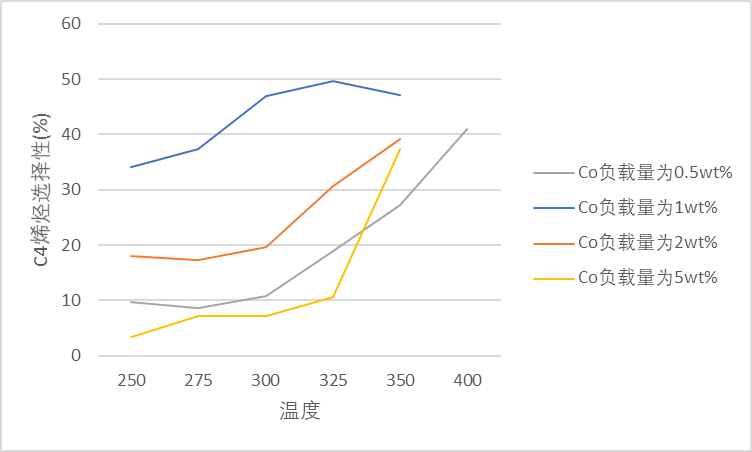
\includegraphics[width=8cm]{200200与1.68Co负载量C4.png}
\end{minipage}
\begin{minipage}[t]{0.48\textwidth}
\centering
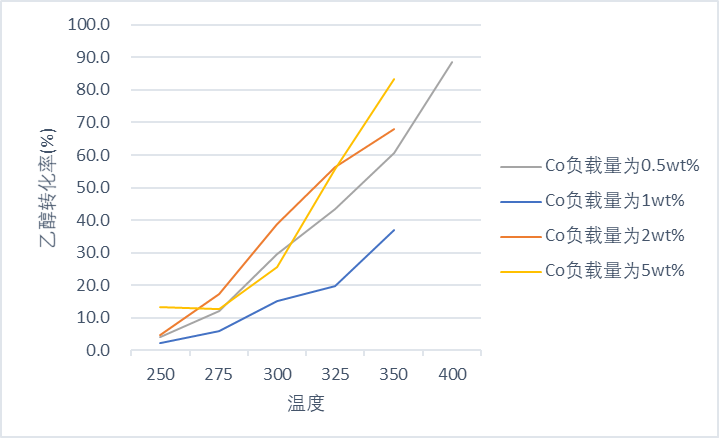
\includegraphics[width=8cm]{200200与1.68Co负载量乙醇.png}
\end{minipage}
\caption{\centering 仅改变Co负载量,C$_4$烯烃选择性和乙醇转化率关于T的折线}
\end{figure}

\begin{figure}[h]
\centering
\begin{minipage}[t]{0.48\textwidth}
\centering
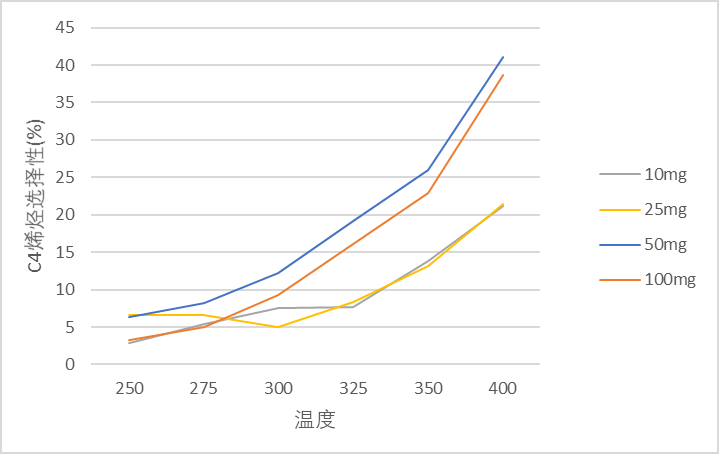
\includegraphics[width=8cm]{一比一不同质量C4.png}
\end{minipage}
\begin{minipage}[t]{0.48\textwidth}
\centering
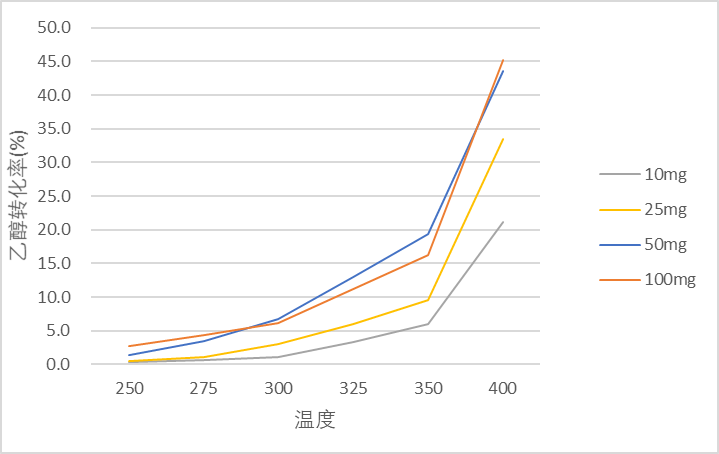
\includegraphics[width=8cm]{一比一不同质量乙醇.png}
\end{minipage}
\caption{\centering 仅改变催化剂质量,C$_4$烯烃选择性和乙醇转化率关于T的折线}
\end{figure}

\begin{figure}[h]
\centering
\begin{minipage}[t]{0.48\textwidth}
\centering
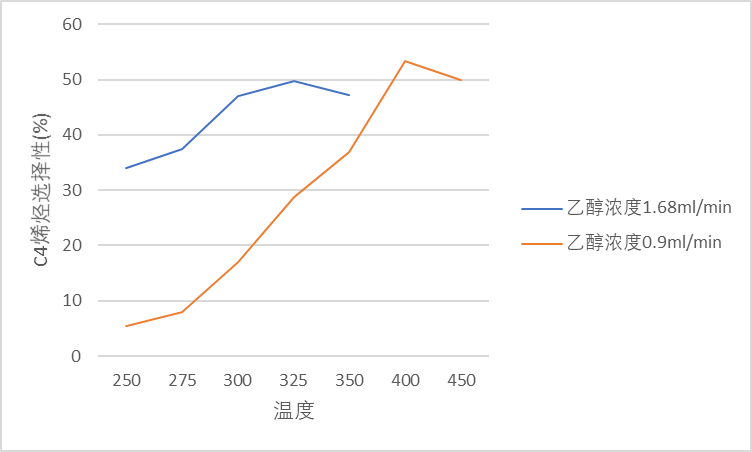
\includegraphics[width=8cm]{200200与1wt乙醇浓度C4.png}
\end{minipage}
\begin{minipage}[t]{0.48\textwidth}
\centering
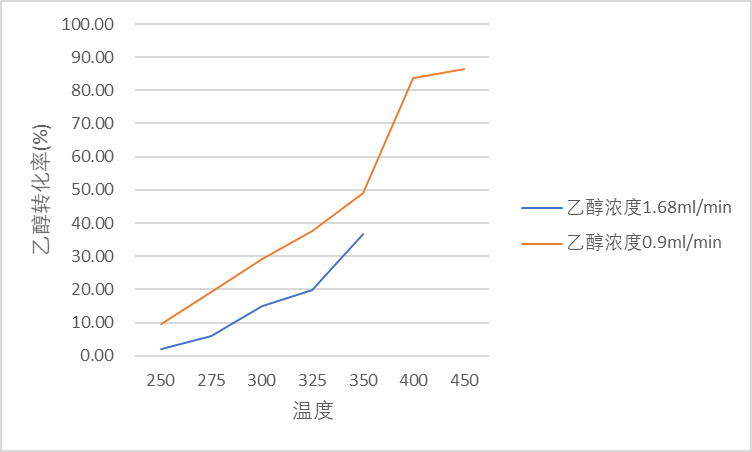
\includegraphics[width=8cm]{200200与1wt乙醇浓度乙醇.png}
\end{minipage}
\caption{\centering 仅改变乙醇浓度,C$_4$烯烃选择性和乙醇转化率关于T的折线}
\end{figure}

\begin{figure}[h]
\centering
\begin{minipage}[t]{0.48\textwidth}
\centering
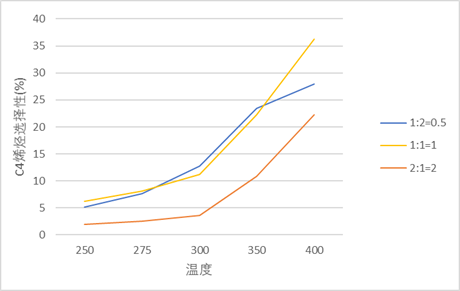
\includegraphics[width=8cm]{100g1wt1.68装料比C4.png}
\end{minipage}
\begin{minipage}[t]{0.48\textwidth}
\centering
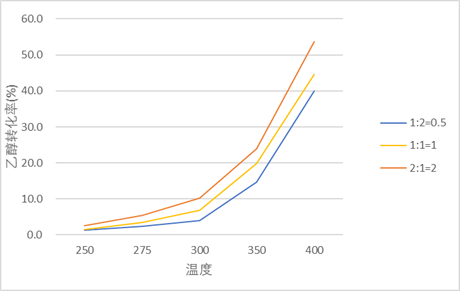
\includegraphics[width=8cm]{100g1wt1.68装料比乙醇.png}
\end{minipage}
\caption{\centering 仅改变装料比,C$_4$烯烃选择性和乙醇转化率关于T的折线}
\end{figure}

\begin{figure}[h]
\centering
\begin{minipage}[t]{0.48\textwidth}
\centering
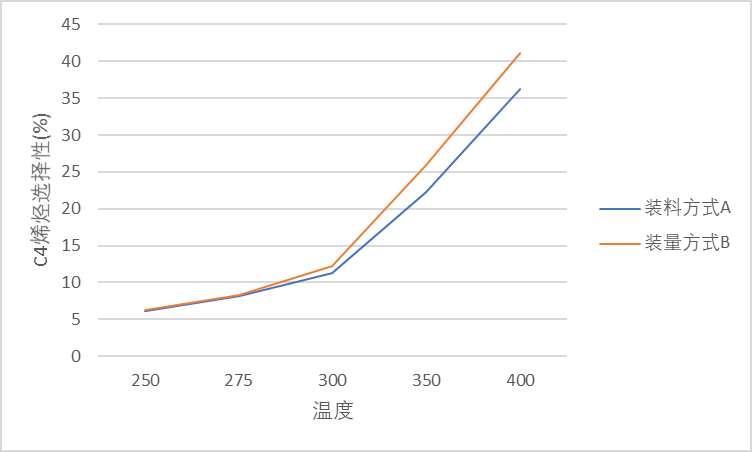
\includegraphics[width=8cm]{50501wt1.68装料C4.png}
\end{minipage}
\begin{minipage}[t]{0.48\textwidth}
\centering
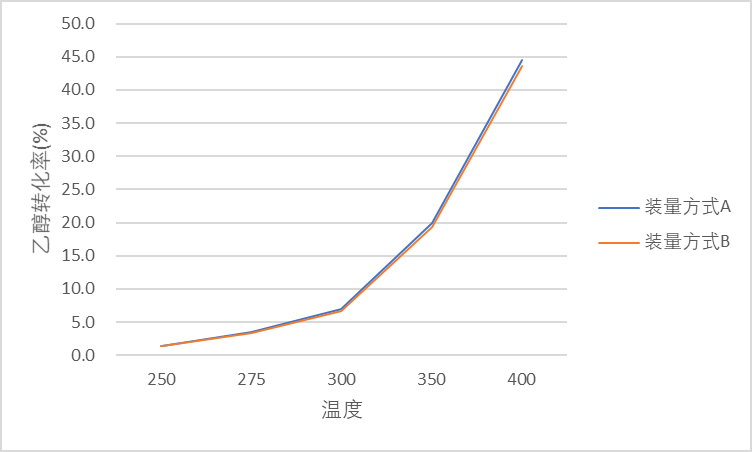
\includegraphics[width=7.5cm]{50501wt1.68装料乙醇.png}
\end{minipage}
\caption{\centering 仅改变装料方式,C$_4$烯烃选择性和乙醇转化率关于T的折线}
\end{figure}
\par 观察五组图片可以得到,当温度小于400$^{\circ}$C时,乙醇转化率与C$_4$烯烃选择性均随着温度升高而显著增加,当温度大于400$^{\circ}$C时(仅有一组实验数据),由于乙烯选择性的增加,C$_4$烯烃选择性出现了下降。
\par 观察图15可以得到,通过纵向对比可知,温度400$^{\circ}$C,Co/SiO$_2$与HAP质量比为200mg:200mg,乙醇浓度1.68ml/min时,当Co负载量从0.5wt$\%$增加到5wt$\%$,C$_4$烯烃选择性百分比呈现先增加后减少的趋势,而乙醇转化率的变化趋势与它不同,当Co负载量为1wt$\%$时,乙醇转化率总体最小,而对于其它负载量,没有明显的关系。
\par 观察图16可以得到,当催化剂装料比1:1时,经各温度时的纵向对比,Co/SiO$_2$装料量越多,乙醇转化率和C$_4$烯烃选择性明显越高,可以猜测它们与Co/SiO$_2$质量呈正向关系。
\par 观察图17可以得到,在相同反应条件下,乙醇浓度较高时的乙醇转化率显著地低于较低时的结果,可以猜测其与乙醇浓度呈负向关系,但是对C$_4$烯烃选择性的影响不明显,甚至可以根据折线图走势猜测,若增加乙醇浓度1.68ml/min的实验样本,温度大于350$^{\circ}$C时,乙醇浓度1.68ml/min的C$_4$烯烃选择性转而低于乙醇浓度0.9ml/min的C$_4$烯烃选择性.
\par 观察图18可以得到,在确定Co/SiO$_2$与HAP总质量为100mg且在反应条件相同时,HAP比Co/SiO$_2$的值越高,乙醇转化率越高,而C$_4$烯烃选择性相反,此时1:1装料比的百分比总体最高,2:1装料比的选择性百分比远低于另外两种情况。
\par 观察图19可以得到,在相同的反应条件下,两种装量方式具有相似的乙醇转化率和C$_4$烯烃选择性,说明装料方式对催化剂的性能并没有显著影响。
~\\
\par 有了上述定性分析的基础,下面考虑利用STATA软件进行多元线性回归,进一步分析各指标对目标对影响情况:
\par 根据上述分析得到的6个指标对附件1中的数据进行整理,将催化剂组合中的变量提取出来,其中,装料方式为A时,设值为1,装料方式为B时,设值为0。将整合好的EXCEL(见附录表:性能数据表)导入STATA软件,利用STATA软件中的$regress$语句回归,回归目标分别为为乙醇转化率($y_1$)与C$_4$烯烃选择性($y_2$),自变量为:装料方式($x_1$)、Co负载量($x_2$)、Co/SiO$_2$质量($x_3$)、装料比($x_4$)、乙醇浓度($x_5$)、温度(T)。在实验后,得到标准化的回归方程如下:
$$y_1=0.091236x_1-0.012322x_2+0.301581x_3+0.055253x_4-0.188642x_5+0.771521T$$
$$y_2=0.136174x_1-0.315466x_2+0.390606x_3-0.086818x_4+0.130576x_5+0.726611T$$
\par 考察上述多元线性回归方程,发现两个函数的拟合优度$R^2\approx 0.8$,在第一个回归方程中Co/SiO$_2$质量($x_3$)、乙醇浓度($x_5$)、温度(T)的系数在95\%的置信水平下显著;在第二个回归方程中装料方式($x_1$)、Co负载量($x_2$)、Co/SiO$_2$质量($x_3$)、乙醇浓度($x_5$)、温度(T)在95\%的置信水平下显著(具体见模型的分析与检验部分),故而可以利用上述函数作为乙醇转化率与C$_4$烯烃选择性关于六项自变量的近似线性函数。根据折线图和函数关系式可以得出,当其他条件不变时,在一定范围内,斜率系数可以表明:
\par 温度对变量影响明显:每升高1个单位,乙醇转化率平均增加0.771521个单位,C$_4$烯烃选择性平均增加0.726611个单位;
\par 同时,两者均随着催化剂质量的增加而增加:Co/SiO$_2$质量每增加1个单位,乙醇转化率约增加0.305181个单位,C$_4$烯烃选择性约增加0.390606个单位;
\par 乙醇转化率随着乙醇浓度的增加而有下降趋势,将乙醇浓度提高1个单位,乙醇转化率平均减少0.188642个单位,C$_4$烯烃选择性平均增加0.130576个单位;
\par 两个方程的$x_1$的系数表示装料方式A和装料方式B时乙醇转化率与C$_4$烯烃选择性的平均差距,如果我们进行装料比、催化剂质量等变量均相同的实验,将催化剂以A和B的方式装料,则A装料实验的乙醇转化率平均比B装料实验高出0.091236个单位,A装料实验的C$_4$烯烃选择性平均比B装料实验高出0.136174个单位;
\par Co负载量的系数均为为负,说明每增加1个单位,乙醇转化率平均减少0.012322个单位,C$_4$烯烃选择性平均增加0.315466个单位,但结合折线图,发现仅负向关系较难解释样本中的现象,尚可确定其为不起到正作用的较为复杂的变量;
\par 在催化剂总量相同时,乙醇转化率随着装料比的增加而增加,C$_4$烯烃选择性大体上与装料比的变化趋势相反:如果装料比提高一个单位,则乙醇转化率平均增加0.055253个单位,C$_4$烯烃选择性平均减少0.086818个单位,但根据折线图综合考量,超过350$^{\circ}$C时,1:1的装料比导致的C$_4$烯烃选择性最大,催化剂具有较好的催化效果。
\subsection{问题三的建模与求解}
\subsubsection{问题三的建模}
与问题二的建模类似,仍然将催化剂组合及其装料方式转化为Co负载量、Co/SiO$_2$质量、Co/SiO$_2$和HAP的装料比、乙醇浓度和装料方式(虚拟变量)五个变量,加上温度共六个解释变量,作为C$_4$烯烃收率大小的影响因素,建立影响C$_4$烯烃收率大小的多元线性回归模型。在刻画Co/SiO$_2$和HAP的转料比与质量时需要两个变量,问题二中使用了Co/SiO$_2$质量与Co/SiO$_2$和HAP的装料比,满足关系式:HAP质量=Co/SiO$_2$质量$\times$装料比,在本题中可以考虑总质量(HAP质量+Co/SiO$_2$质量)与装料比,替代上述两个量用于描述Co/SiO$_2$和HAP的装料比与质量。再考虑350$^{\circ}$C以下,选择催化剂与温度使得C$_4$烯烃收率最大的问题:去除350度以上数据后再进行回归分析,得到在350度以下对C$_4$烯烃收率较为显著的影响因子。

进行回归后观察各变量的的显著性与系数,结合实际考察各变量对C$_4$烯烃收率大小的影响。若显著性较差,可以考虑对各变量进行处理后再进行回归,最终得到较好的回归方程。

\subsubsection{问题三的求解}
根据控制变量的原理,利用EXCEL作出仅改变一个变量时实验C$_4$烯烃收率随温度的变化。
\begin{figure}[h]
\centering
\begin{minipage}[t]{0.48\textwidth}
\centering
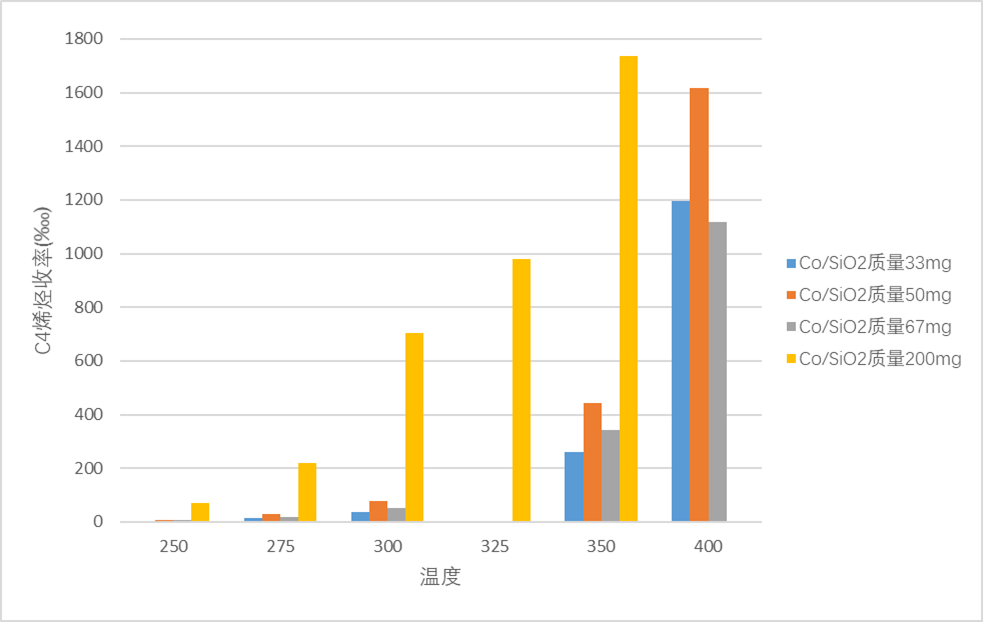
\includegraphics[width=7cm]{CoSiO2质量1wt1.68ml.png}
\caption{仅改变CoSiO$_2$质量C$_4$烯烃收率与温度的关系}
\end{minipage}
\begin{minipage}[t]{0.48\textwidth}
\centering
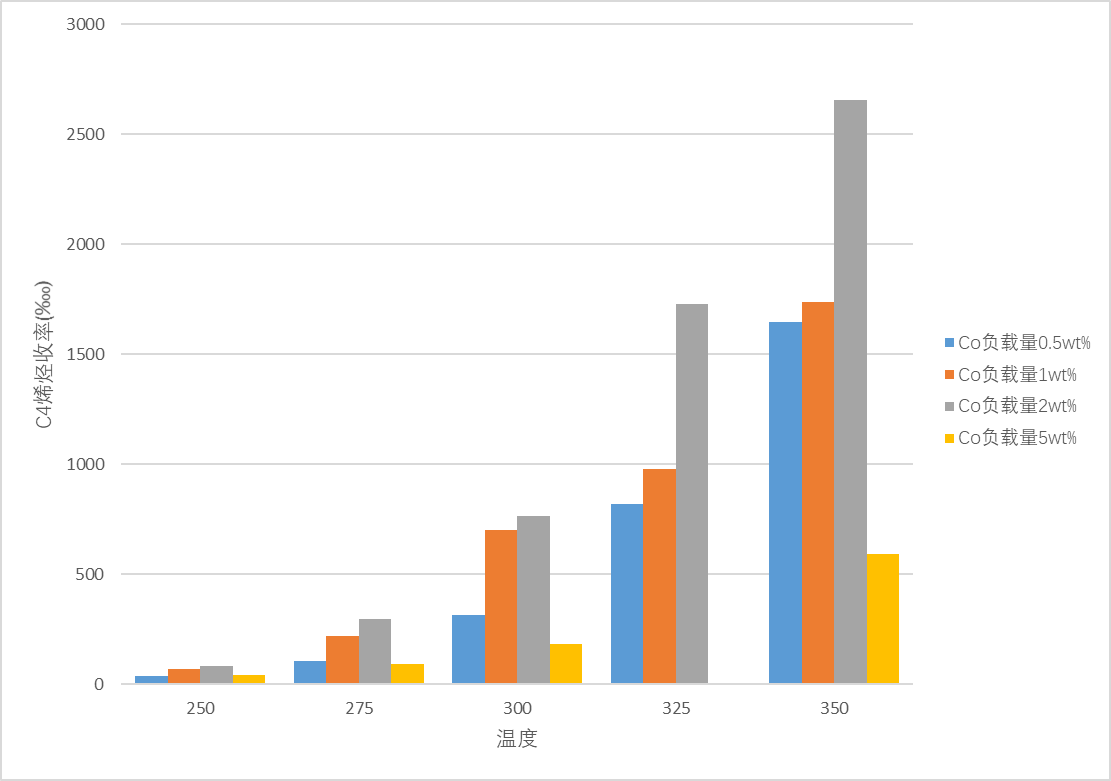
\includegraphics[width=7cm]{Co负载量1.68ml200400.png}
\caption{仅改变Co负载量C$_4$烯烃收率与温度的关系}
\end{minipage}
\end{figure}

\begin{figure}[h]
\centering
\begin{minipage}[t]{0.48\textwidth}
\centering
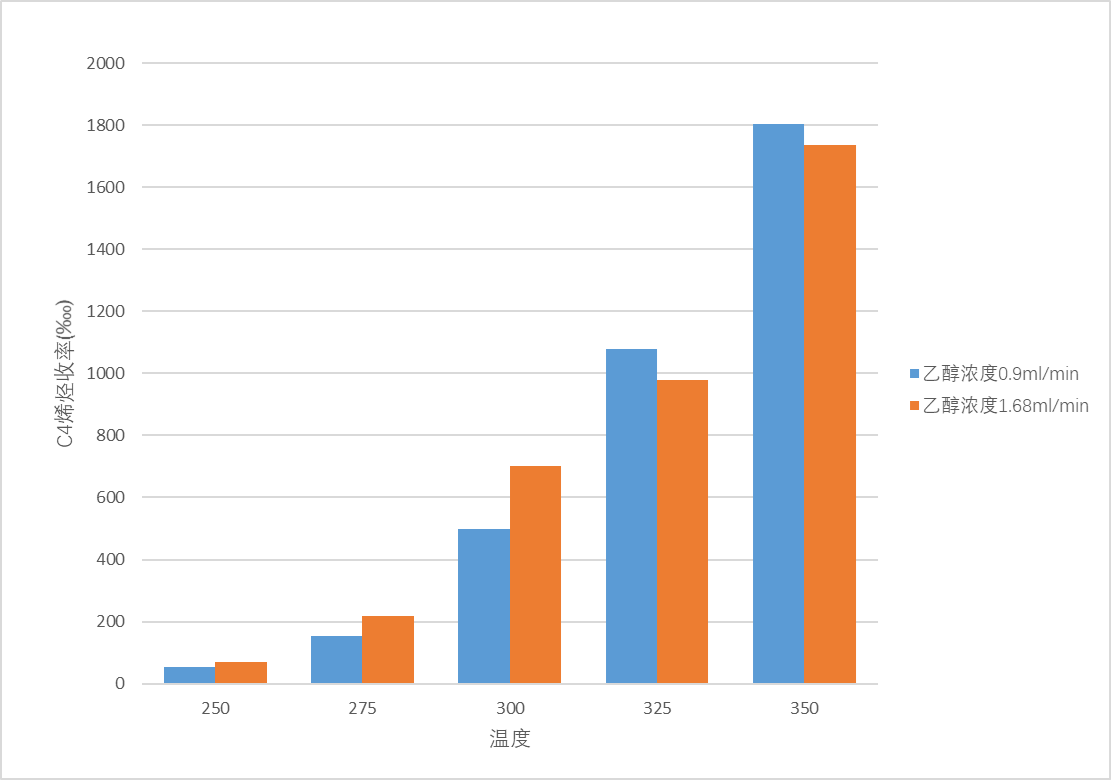
\includegraphics[width=7cm]{乙醇三百度1wt200400.png}
\caption{仅改变乙醇浓度C$_4$烯烃收率与温度的关系}
\end{minipage}
\begin{minipage}[t]{0.48\textwidth}
\centering
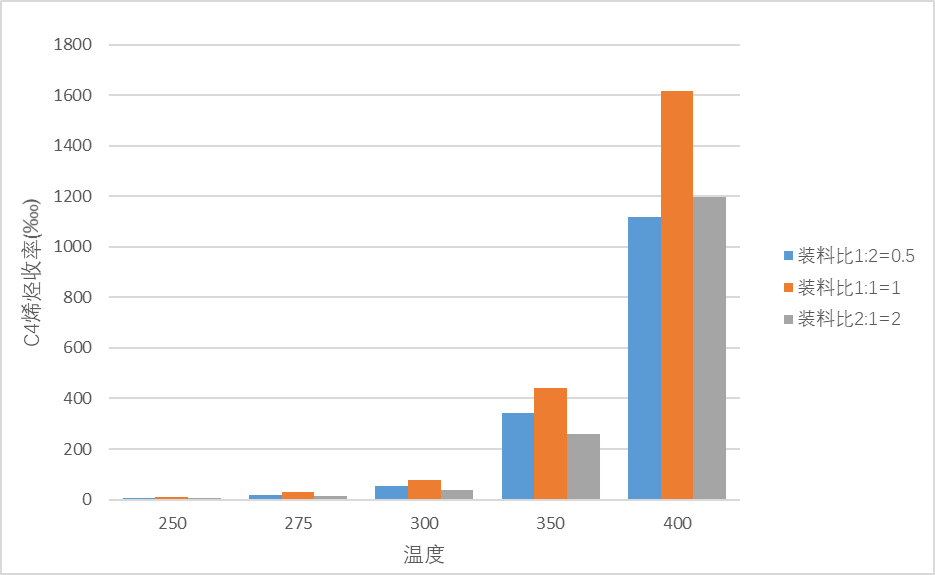
\includegraphics[width=7cm]{装料比总质量100mg.png}
\caption{仅改变装料比C$_4$烯烃收率与温度的关系}
\end{minipage}
\end{figure}
\vspace*{150pt}



观察六张图片,考察C$_4$烯烃收率与各变量的关系,发现控制催化剂不变时,几乎所有实验中C$_4$烯烃收率均随温度升高而有明显上升,这与问题二中我们研究所得的结论相符(乙醇转化率与烯烃选择性在同种催化剂下均随温度升高而增大)。

观察图10,发现Co/SiO$_2$质量为200mg时,C$_4$烯烃收率最大。控制装料比相同(1:1),Co/SiO$_2$质量分别为200mg与50mg时,C$_4$烯烃收率有显著差别,Co/SiO$_2$质量越大(即总质量越大),C$_4$烯烃收率越高。

观察图10,发现控制其他变量相同时,Co负载量为1wt\%时,C$_4$烯烃收率最大,并且C$_4$烯烃收率随Co负载量与1wt\%的差异增大而减小。

观察图10,发现乙醇浓度在不同温度下大小关系并不一致,并且差异不大,猜测乙醇浓度对C$_4$烯烃收率的影响不大。

观察图10,发现控制总质量相同,仅改变装料比时,装料比为1:1且温度为400度时,C$_4$烯烃收率明显大于其它两类,猜测装料比为1:1时C$_4$烯烃收率有最大值。

观察图10,发现装料方式对于C$_4$烯烃收率影响较小,装料方式A对应的C$_4$烯烃收率略高于装料方式B。

观察图10,发现总质量对C$_4$烯烃收率有较明显影响,即总质量越大C$_4$烯烃收率越大,这与上述对CoSiO$_2$质量的分析有关并且一致。
~\\
\par 有了上述分析的基础,再考虑进行多元线性回归,获得各解释变量与C$_4$烯烃收率较为准确的关系。考虑以Co负载量、Co/SiO$_2$和HAP的装料比、乙醇浓度、装料方式(虚拟变量)和温度作为解释变量对C$_4$烯烃收率进行回归。在EXCEL中对数据进行预处理后,在STATA中导入变量并计算C$_4$烯烃收率,利用STATA中$regress$语句回归,回归目标为C$_4$烯烃收率($z$),自变量为:装料方式($x_1$)、Co负载量($x_2$)、装料比($x_3$)、Co/SiO$_2$质量($x_4$)、乙醇浓度($x_5$)、温度($T$),得到线性多元回归方程系数如下表:
% Table generated by Excel2LaTeX from sheet 'Sheet4'
% Table generated by Excel2LaTeX from sheet 'Sheet1'
\begin{table}[htbp]
  \centering
  \caption{C$_4$烯烃收率关于装料方式等的回归结果}
    \begin{tabular}{ccccccc}
    \toprule[2pt]
    C$_4$烯烃收率 & 系数    & 标准误差  & $t$ & $P>|t|$ & \multicolumn{2}{p{10.225em}}{[95\%置信区间]} \\
    \midrule
    装料方式  & 158.30180  & 126.51300  & 1.25  & 0.214 & -92.6361 & 409.2398 \\
    Co负载量 & -87.77591  & 47.46761  & -1.85 & 0.067 & -181.9277 & 6.375873 \\
    CoSiO$_2$质量 & 4.19203  & 0.86203  & 4.86  & 0.000 & 2.482194 & 5.901855 \\
    装料比   & 15.31978  & 215.91570  & 0.07  & 0.944 & -412.948 & 443.5876 \\
    乙醇浓度  & -113.51390  & 106.91380  & -1.06 & 0.291 & -325.577 & 98.54916 \\
    温度    & 13.46720  & 0.99419  & 13.55 & 0.000 & 11.49523 & 15.43918 \\
    常数项   & -3878.95000  & 441.06640  & -8.79 & 0.000 & -4753.803 & -3004.097 \\
    \bottomrule[2pt]
    \end{tabular}%
  \label{tab:addlabel}%
\end{table}%

观察该表可知,将各变量作为解释变量直接进行回归的效果并不好:装料方式、Co负载量、装料比、乙醇浓度在95\%的置信水平下均不显著,进行怀特检验后发现存在异方差,考虑使用最小二乘法与稳健的标准误\cite{article2}:
% Table generated by Excel2LaTeX from sheet 'Sheet1'
\begin{table}[htbp]
  \centering
  \caption{C$_4$烯烃收率关于装料方式等使用稳健的标准误的回归结果}
    \begin{tabular}{ccccccc}
    \toprule[2pt]
    C$_4$烯烃收率 & 系数    & 稳健的标准误 & $t$ & $P>|t|$ & \multicolumn{2}{p{10.225em}}{[95\%置信区间]} \\
    \midrule
    装料方式  & 158.30180  & 98.61435  & 1.61  & 0.112 & -37.29927 & 353.9029 \\
    Co负载量 & -87.77591  & 56.25768  & -1.56 & 0.122 & -199.3627 & 23.81093 \\
    CoSiO$_2$质量 & 4.19203  & 0.90661  & 4.62  & 0.000 & 2.393769 & 5.99028 \\
    装料比   & 15.31978  & 169.36770  & 0.09  & 0.928 & -320.6202 & 351.2598 \\
    乙醇浓度  & -113.51390  & 105.29180  & -1.08 & 0.284 & -322.3598 & 95.33192 \\
    温度    & 13.46720  & 1.35176  & 9.96  & 0.000 & 10.78599 & 16.14842 \\
    常数项   & -3878.95000  & 497.91370  & -7.79 & 0.000 & -4866.56 & -2891.341 \\
    \bottomrule[2pt]
    \end{tabular}%
  \label{tab:addlabel}%
\end{table}%

发现显著性变化不大,下面考虑对各变量进行预处理后再进行回归。

根据上述六张图片的分析,并且装料方式显然已不显著,故考虑将Co负载量、装料比、乙醇浓度分别转换为三者与2wt\%、1、0.9ml/min的距离,可以通过差的绝对值、差的平方、差值开根等进行刻画,再结合温度与总质量进行回归。

在进行多次试验后得到如下两次较好的回归结果(系数为标准化后的系数):
\begin{equation}
\begin{aligned}
\nonumber
z&=-0.039\cdot |x_2-2|+0.304x_3(x_4+1)-0.023\cdot |x_4-1|-0.126\cdot |x_5-0.9|+0.738T\\
z&=-0.039\cdot |x_2-2|+0.305x_3(x_4+1)-0.021\cdot |x_4-1|^2-0.126\cdot |x_5-0.9|+0.738T
\end{aligned}
\end{equation}
回归方程中温度(T)、总质量($x_3(x_4+1)$)以及乙醇浓度与0.9的距离($|x_5-0.9|$)的系数在95\%的置信水平下显著异于0,故而下面探讨这几种变量对于C$_4$烯烃收率的影响。根据柱状图和函数关系式可以得出,当其他条件不变时,在一定范围内,斜率系数可以表明:
\par 温度对变量影响明显:每升高1个单位,C$_4$烯烃收率平均增加0.738个单位;
\par 同时,C$_4$烯烃收率随催化剂质量的增加而增加:总质量每增加1个单位,C$_4$烯烃收率约增加0.304个单位;
\par C$_4$烯烃收率随着乙醇浓度与0.9距离的增加而有下降趋势,将乙醇浓度与0.9的距离提高1个单位,C$_4$烯烃收率平均减少0.126个单位;
\par Co负载量与2的距离的系数为负,说明 Co负载量与2的距离每增加1个单位,乙醇转化率平均减少0.039个单位;
\par 查阅参考文献可得,装料比为1:1时,C$_4$烯烃收率有最优值,观察柱状图亦可得到,装料方式B的C$_4$烯烃收率略高于装料方式A。

故而考虑选取装料方式A、Co负载量为2wt\%时、装料比为1:1、总质量为400mg(Co/SiO$_2$质量为200mg)、乙醇浓度为0.9ml/min、温度为400度时,C$_4$烯烃收率有最大值。
~\\
\input{问题三求解后半部分.txt}
\subsection{问题四的求解}
\input{问题四的求解.txt}
\section{模型的分析与检验}
\par 拟合优度 $R^2$,也称可决系数,通常用于评价回归结果或者拟合函数对参数成线性时的拟合结果。$R^2$ 的计算公式如下:
\begin{equation}
\begin{aligned}
\nonumber
SST &= \sum_{i=1}^{n}(y_i-\overline{y})^2\\
SSE &= \sum_{i=1}^{n}(y_i-\hat{y}_i)^2\\
SSR &= \sum_{i=1}^{n}(\hat{y}_i-\overline{y})^2
\end{aligned}
\end{equation}
$$R^2=\frac{SSR}{SST}=1-\frac{SSE}{SST}.$$
\par 其中,$SST$ 称为总体平方和,$SSE$ 称为误差平方和,$SSR$ 称为回归平方和。$R^2$ 越接近 $1$,说明误差平方和越接近 $0$,说明拟合效果越好。
\par 均方根误差(RMSE)的计算公式如下:
$$ {\rm RMSE}=\sqrt{{\rm MSE}}=\sqrt{\frac{1}{n}SSE}=\sqrt{\frac{1}{n}\sum_{i=1}^{n}(y_i-\hat{y}_i)^2}$$

\subsection{问题一模型的分析与检验}
\input{模型一分析与检验.txt}

\subsection{问题二模型的分析与检验}
\par 在第二个问题的求解中,利用STATA对乙醇转化率与C$_4$烯烃选择性和分析出的六个变量进行多元线性回归。下面基于回归得到的各项指标,对回归结果进行分析与检验。
\par 由结果可知,在对乙醇转化率的回归模型中,拟合优度$R^2$=0.8021,校正的拟合优度Adjusted $R^2$=0.7905;在对C$_4$烯烃选择性的回归模型中,拟合优度$R^2$=0.7486,校正的拟合优度Adjusted $R^2$=0.7338。调整后的$R^2$越大,拟合效果越好。本题中的回归属于解释型的回归,更多关注的是模型整体和回归参数的显著性如何。
\par 接下来考虑回归方程的显著性,研究弃真概论F值。乙醇转化率的回归模型中的F=68.91,C$_4$烯烃选择性的回归模型中的F=50.63,均大于F检验临界值,因此回归方程显著,解释变量和被解释变量间存在明显函数关系。
\par 下表中给出了两个回归模型中对6个自变量的偏回归系数的T检验结果。从表中可知,在对乙醇转化率的解释中,概率p都小于显著性水平0.05的变量是Co/SiO$_2$质量、乙醇浓度和温度;在对C$_4$烯烃选择性的解释中,显著性水平小于0.05的变量是Co负载量、Co/SiO$_2$质量和温度。因此认为这些相关系数$\beta$显著地不为0,与因变量线性相关水平显著。
% Table generated by Excel2LaTeX from sheet 'Sheet3'
\begin{table}[htbp]
  \centering
  \caption{乙醇转化率关于装料方式等的回归结果}
    \begin{tabular}{cccccccc}
    \toprule[2pt]
    乙醇转化率 & 系数 & 标准误差  &  $t$    & $P>|t|$ & \multicolumn{2}{c}{ [95$\%$ 的置信区间]} & 标准化后的系数 \\
    \midrule
    装料方式  & 4.336637  & 2.471729  & 1.75  & 0.082  & -0.56603  & 9.23930  & 0.091236  \\
     Co负载量 & -0.239550  & 0.927391  & -0.26  & 0.797  & -2.07903  & 1.59993  & -0.012322  \\
     Co/SiO$_2$质量  & 0.097801  & 0.016842  & 5.81  & 0.000  & 0.06440  & 0.13121  & 0.301581  \\
     装料比  & 5.170628  & 4.218421  & 1.23  & 0.223  & -3.19659  & 13.53785  & 0.055253  \\
     乙醇浓度  & -8.227098  & 2.088813  & -3.94  & 0.000  & -12.37025  & -4.08395  & -0.188642  \\
     温度   & 0.339908  & 0.019424  & 17.50  & 0.000  & 0.30138  & 0.37844  & 0.771521  \\
     常数项  & -89.987520  & 8.617269  & -10.440  & 0.000  & -107.07980  & -72.89520  &  \\
    \bottomrule[2pt]
    \end{tabular}%
  \label{tab:addlabel}%
\end{table}%


% Table generated by Excel2LaTeX from sheet 'regress1'
\begin{table}[htbp]
  \centering
  \caption{C$_4$烯烃选择性关于装料方式等的回归结果}
    \begin{tabular}{cccccccc}
    \toprule[2pt]
     C$_4$烯烃选择性 & 系数 & 标准误差  &  $t$    & $P>|t|$ & \multicolumn{2}{c}{ [95\% 的置信区间]} & 标准化后的系数 \\
    \midrule
    装料方式  & 3.799291  & 1.635252  & 2.32  & 0.022  & 0.5557775  & 7.0428050  & 0.136174  \\
     Co负载量 & -3.599927  & 0.613546  & -5.87  & 0.000  & -4.8168920  & -2.3829630  & -0.315466  \\
     Co/SiO$_2$质量 & 0.074353  & 0.011142  & 6.67  & 0.000  & 0.0522526  & 0.0964536  & 0.390606  \\
     装料比  & -4.768830  & 2.790832  & -1.71  & 0.091  & -10.3044300  & 0.7667717  & -0.086818  \\
     乙醇浓度  & 3.342660  & 1.381921  & 2.42  & 0.017  & 0.6016259  & 6.0836940  & 0.130576  \\
     温度   & 0.187904  & 0.012851  & 14.62  & 0.000  & 0.1624146  & 0.2133925  & 0.726611  \\
     常数项  & -46.906050  & 5.701031  & -8.230  & 0.000  & -93.8121000  & -35.5980800  &  \\
    \bottomrule[2pt]
    \end{tabular}%
  \label{tab:addlabel}%
\end{table}%

\par 在问题二的模型建立中,我们假定了扰动项$\xi$同方差和无自相关两条性质,而本文中的横截面数据很容易出现异方差的现象,因此我们利用怀特检验(White Test)检验是否存在异方差,防止方差较大的扰动项对我们模型稳定性的破坏。原假设$H_0$=不存在异方差,在回归结束后利用STATA命令:$estat\,imest,white$。乙醇转化率的回归模型得到怀特检验的统计量$chi2(21)$=49.09,且在C$_4$烯烃选择性的回归模型得到怀特检验的统计量$chi2(21)$=53.60,说明存在异方差。下面考虑使用最小二乘法与稳健的标准误对模型进行回归,得到下表,显著性变量不变:
~\\
% Table generated by Excel2LaTeX from sheet 'Sheet3'
\begin{table}[htbp]
  \centering
  \caption{使用稳健的标准误后乙醇转化率关于装料方式等的回归结果}
    \begin{tabular}{cccccccc}
    \toprule[2pt]
    乙醇转化率 & 系数 & 稳健的标准误 &  $t$    & $P>|t|$ & \multicolumn{2}{c}{ [95\% 置信区间]} & 标准化后的系数 \\
    \midrule
    装料方式  & 4.336637  & 2.079950  & 2.08  & 0.040  & 0.21107  & 8.46221  & 0.091236  \\
     Co负载量 & -0.239550  & 1.039114  & -0.23  & 0.818  & -2.30063  & 1.82153  & -0.012322  \\
     CoSiO2质量  & 0.097801  & 0.019215  & 5.09  & 0.000  & 0.05969  & 0.13591  & 0.301581  \\
     装料比  & 5.170628  & 2.660127  & 1.94  & 0.055  & -0.10572  & 10.44698  & 0.055253  \\
     乙醇浓度  & -8.227098  & 2.645042  & -3.11  & 0.002  & -13.47353  & -2.98067  & -0.188642  \\
     温度   & 0.339908  & 0.020754  & 16.38  & 0.000  & 0.29874  & 0.38107  & 0.771521  \\
     常数项  & -89.987520  & 9.260551  & -9.720  & 0.000  & -108.35580  & -71.61926  &  \\
    \bottomrule[2pt]
    \end{tabular}%
  \label{tab:addlabel}%
\end{table}%


% Table generated by Excel2LaTeX from sheet 'regress1'
\begin{table}[htbp]
  \centering
  \caption{使用稳健的标准误后C$_4$烯烃选择性关于装料方式等的回归结果}
    \begin{tabular}{ccccccccc}
    \toprule[2pt]
    C_4烯烃选择性 &系数 & 稳健的标准误 &  $t$    & $P>|t|$ & \multicolumn{2}{c}{ [95\% 置信区间]} & 标准化后的系数 \\
    \midrule
    装料方式  & 3.799291  & 1.212365  & 3.13  & 0.002  & 1.3945700  & 6.2040120  & 0.136174  \\
     Co负载量 & -3.599927   & 0.733714  & -4.91  & 0.000  & -5.0552460  & -2.1446090  & -0.315466  \\
     CoSiO2质量  & 0.074353  & 0.013918  & 5.34  & 0.000  & 0.0467467  & 0.1019595  & 0.390606  \\
     装料比  & -4.768830   & 1.982468  & -2.41  & 0.018  & -8.7010460  & -0.8366141  & -0.086818  \\
     乙醇浓度  & 3.342660   & 1.422809  & 2.35  & 0.021  & 0.5205246  & 6.1647960  & 0.130576  \\
     温度   & 0.187904   & 0.012479  & 15.06  & 0.000  & 0.1631509  & 0.2126562  & 0.726611  \\
     常数项  & -46.906050  & 4.714759  & -9.950  & 0.000  & -56.2577500  & -37.5543500  &  \\
    \bottomrule[2pt]
    \end{tabular}%
  \label{tab:addlabel}%
\end{table}%

\par 为了防止自变量之间存在多重共线性而导致的$(X^{T}X)^{-1}$的不存在和参数的难以识别,虽然本次实验中选取的解释变量看上去独立,不存在任何关系,但为了保证检验的完整性,下面我们通过方差膨胀因子VIF来检验:在回归结束以后,利用STATA软件各自变脸的VIF命令:$estat\,vif$,由于两次模型中自变量相同,所以得到同一组VIF数据,见下表。从表中可见,各变量的VIF值均远小于10,说明构建模型的变量之间相关性很小。
% Table generated by Excel2LaTeX from sheet 'Sheet1'
\begin{table}[htbp]
  \centering
  \caption{装料方式等变量间的回归的多重共线性检验}
    \begin{tabular}{cccccccr}
    \toprule[2pt]
    变量    & 装料方式  & Co/SiO2 质量 & 乙醇浓度  & Co负载量 & 装料比   & 温度    & \multicolumn{1}{c}{Mean VIF} \\
    \midrule
    VIF   & 1.39  & 1.39  & 1.18  & 1.17  & 1.05  & 1     & \multicolumn{1}{c}{1.2} \\
    1/VIF & 0.71742 & 0.719289 & 0.845701 & 0.852538 & 0.954699 & 0.998048 &  \\
    \bottomrule[2pt]
    \end{tabular}%
  \label{tab:addlabel}%
\end{table}%
\subsection{问题三模型的分析与检验}
\par 在第三个问题的求解中,利用STATA对C$_4$烯烃收率和分析出的六个变量进行多元线性回归。下面基于回归得到的各项指标,对回归结果进行分析与检验。
\par 首先对温度不设限制的模型进行分析与检验:
\par 在变量选择同问题二的回归初尝试中,拟合优度$R^2$=0.6947,校正的拟合优度Adjusted $R^2$=0.6768,拟合优度不高。接下来看模型整体和回归参数的显著性:弃真概论F=38.69,大于F检验的临界值,因此此回归方程显著,自变量与因变量间函数关系明显;下表中给出了回归模型中对6个自变量的偏回归系数的T检验结果,其中,装料方式、Co负载量、装料比和乙醇浓度在95$\%$的置信区间下均不显著,因此本次回归效果并不理想。
\begin{table}[htbp]
  \centering
  \caption{C$_4$烯烃收率关于装料方式等的回归结果}
    \begin{tabular}{ccccccc}
    \toprule[2pt]
    C$_4$烯烃收率 & 系数    & 标准误差  & $t$ & $P>|t|$ & \multicolumn{2}{p{10.225em}}{[95\%置信区间]} \\
    \midrule
    装料方式  & 158.30180  & 126.51300  & 1.25  & 0.214 & -92.6361 & 409.2398 \\
    Co负载量 & -87.77591  & 47.46761  & -1.85 & 0.067 & -181.9277 & 6.375873 \\
    CoSiO$_2$质量 & 4.19203  & 0.86203  & 4.86  & 0.000 & 2.482194 & 5.901855 \\
    装料比   & 15.31978  & 215.91570  & 0.07  & 0.944 & -412.948 & 443.5876 \\
    乙醇浓度  & -113.51390  & 106.91380  & -1.06 & 0.291 & -325.577 & 98.54916 \\
    温度    & 13.46720  & 0.99419  & 13.55 & 0.000 & 11.49523 & 15.43918 \\
    常数项   & -3878.95000  & 441.06640  & -8.79 & 0.000 & -4753.803 & -3004.097 \\
    \bottomrule[2pt]
    \end{tabular}%
  \label{tab:addlabel}%
\end{table}%
\par 根据结果和文献资料,我们剔除装料方式这一不显著的变量,其余变量中,我们作出适当改进并且引入了二次项:Co负载量转化为Co负载量与2的距离、Co/SiO$_2$质量转化为总质量、装料比分别转化为装料比与1的距离和距离的平方、乙醇浓度转化为乙醇浓度为0.9的距离。改进模型后的拟合优度$R^2$分别为0.6934和0.6933,F分别为46.58和46.56,均大于F检验的临界值,说明该回归拟合优度不高但回归方程显著;下面分析回归参数的显著性,结果如下表,发现:不显著的解释变量减少,剩下Co负载量与2的距离,分别地装料比与1距离和距离的平方不显著。
% Table generated by Excel2LaTeX from sheet 'Sheet1'
\begin{table}[htbp]
  \centering
  \caption{C$_4$烯烃收率关于装料比与1的距离等变量的回归结果}
    \begin{tabular}{cccccc}
    \toprule[2pt]
    C$_4$烯烃收率 & 系数    & 标准误差 & $t$ & $P>|t|$ &标准化后的系数 \\
    \midrule
    Co负载量 & -53.86023 & 77.68063  & -0.69 & 0.490 & -0.03909  \\
    总质量   & 2.039664  & 0.38868  & 5.25  & 0.000 & 0.30444  \\
    装料比与1的距离 & -93.50157 & 224.14630  & -0.42 & 0.677 & -0.02334  \\
    乙醇浓度与0.9的距离 & -340.3238 & 158.26870  & -2.15 & 0.034 & -0.12609  \\
    温度    & 13.40681  & 0.99288  & 13.50 & 0.000 & 0.73845  \\
    常数项   & -3723.666 & 361.88430  & -10.29 & 0.000 &  \\
    \bottomrule[2pt]
    \end{tabular}%
  \label{tab:addlabel}%
\end{table}%
% Table generated by Excel2LaTeX from sheet 'Sheet1'
\begin{table}[htbp]
  \centering
  \caption{C$_4$烯烃收率关于装料比与1的距离的平方等变量的回归结果}
    \begin{tabular}{cccccc}
    \toprule[2pt]
    C$_4$烯烃收率 & 系数    & 标准误差   & $t$ & $P>|t|$ &标准化后的系数 \\
    \midrule
    Co负载量 & -53.42792 & 77.65723  & -0.69 & 0.493 & -0.038779  \\
    总质量   & 2.046101  & 0.38715  & 5.29  & 0.000 & 0.305399  \\
    装料比与1的距离的平方 & -87.20724 & 232.57570  & -0.37 & 0.708 & -0.020875  \\
    乙醇浓度与0.9的距离 & -340.72 & 158.27950  & -2.15 & 0.034 & -0.126240  \\
    温度    & 13.4069  & 0.99304  & 13.50 & 0.000 & 0.738453  \\
    常数项   & -3726.499 & 361.61100  & -10.31 & 0.000 &  \\
    \bottomrule[2pt]
    \end{tabular}%
  \label{tab:addlabel}%
\end{table}%

\par 下面类似问题二,我们利用检验(White Test)检验是否存在异方差,在回归结束后利用STATA命令:$estat\,imest,white$,得到怀特检验统计量$chi2(17)$均为53.23,否定了原假设,说明存在异方差。所以我们使用OLS+稳健的标准误来解决异方差问题,利用STATA命令:$regress\,y\,x_1,...,x_k,robust$,得到下表,显著性参量不变。
\vspace*{30pt}
% Table generated by Excel2LaTeX from sheet 'Sheet1'
\begin{table}[htbp]
  \centering
  \caption{使用稳健的标准误后C$_4$烯烃收率关于装料比与1的距离等变量的回归结果}
    \begin{tabular}{ccccccc}
    \toprule[2pt]
    C$_4$烯烃收率 & 系数    & 稳健的标准误 & $t$ & $P>|t|$ & \multicolumn{2}{p{10em}}{[95\%置信区间]} \\
    \midrule
    Co负载量 & -53.42792 & 92.40445 & -0.58 & 0.561 & -237.1227 & 129.4022 \\
    总质量   & 2.046101  & .4240847 & 4.81  & 0.000 & 1.198592 & 2.880736 \\
    装料比与1的距离 & -87.20724 & 165.5944 & -0.56 & 0.574 & -421.919 & 234.9158 \\
    乙醇浓度与0.9的距离 & -340.72 & 168.9822 & -2.01 & 0.047 & -675.4602 & -5.187478 \\
    温度    & 13.4069  & 1.308772 & 10.24 & 0.000 & 10.81117 & 16.00245 \\
    常数项   & -3726.499 & 438.3132 & -8.50 & 0.000 & -4592.957 & -2854.375 \\
    \bottomrule[2pt]
    \end{tabular}%
  \label{tab:addlabel}%
\end{table}%
% Table generated by Excel2LaTeX from sheet 'Sheet1'
\begin{table}[htbp]
  \centering
  \caption{使用稳健的标准误后C$_4$烯烃收率关于装料比与1的距离的平方等变量的回归结果}
    \begin{tabular}{ccccccc}
    \toprule[2pt]
    C$_4$烯烃收率 & 系数    & 稳健的标准误 & $t$ & $P>|t|$ & \multicolumn{2}{p{10em}}{[95\%置信区间]} \\
    \midrule
    Co负载量 & -53.42792 & 92.37342  & -0.58 & 0.564 & -236.6288 & 129.773 \\
    总质量   & 2.046101  & .4225174  & 4.84  & 0.000 & 1.208137 & 2.884064 \\
    装料比与1的距离的平方 & -87.20724 & 171.3969  & -0.51 & 0.612 & -427.1326 & 252.7181 \\
    乙醇浓度与0.9的距离 & -340.72 & 168.9499  & -2.02 & 0.046 & -675.7923 & -5.647712 \\
    温度    & 13.4069  & 1.309184  & 10.24 & 0.000 & 10.81044 & 16.00336 \\
    常数项   & -3726.499 & 438.2984  & -8.50 & 0.000 & -4595.76 & -2857.237 \\
    \bottomrule[2pt]
    \end{tabular}%
  \label{tab:addlabel}%
\end{table}%
\par 为了保证检验的完整性,下面我们通过方差膨胀因子VIF来检验变量之间是否存在多重共线性:
% Table generated by Excel2LaTeX from sheet 'Sheet1'
\begin{table}[htbp]
  \centering
  \caption{总质量等变量间的回归的多重共线性检验}
    \begin{tabular}{cccccccc}
    \toprule[2pt]
    变量    & 装料方式  & Co/SiO$_2$质量 & |装料比与1|$^{\frac{1}{4}}$ & |Co负载量-1| & 乙醇浓度  & 温度    & Mean VIF \\
    \midrule
    VIF   & 1.75  & 1.57  & 1.35  & 1.32  & 1.23  & 1     & 1.37 \\
    1/VIF & 0.569992 & 0.638941 & 0.743276 & 0.755805 & 0.815728 & 0.99614 &  \\
    \bottomrule[2pt]
    \end{tabular}%
  \label{tab:addlabel}%
\end{table}%
\par 从表中可见,各变量的VIF值均远小于10,说明构建模型的变量之间相关性很小。

\par 接下来筛选温度低于350$^{\circ}$C的数据后,对模型进行分析检验:
\par 经过尝试,我们在自变量中引入了四次根项等非线性项:装料方式、Co负载量与2的距离、装料比与1的距离的$\frac{1}{4}$次方、Co/SiO$_2$质量、乙醇浓度和温度。对这些变量进行标准化多元线性回归后,首先利用怀特检验(White Test)检验是否存在异方差,得到怀特检验统计量$chi2(21)=38$,否定原假设,存在异方差现象,所以使用OLS+稳健的标准误解决异方差问题,得到下表的回归参数。
\clearpage
此时,在95$\%$的置信区间下,仅乙醇浓度这一自变量不显著。同样的,为了保证检验的完整性,下面我们通过方差膨胀因子VIF来检验变量之间是否存在多重共线性:
% Table generated by Excel2LaTeX from sheet 'Sheet1'
\begin{table}[htbp]
  \centering
  \caption{装料方式等变量间的回归的多重共线性检验}
    \begin{tabular}{cccccccc}
    \toprule[2pt]
    变量    & 装料方式  & Co/SiO$_2$质量 & |装料比与1|$^{\frac{1}{4}}$ & |Co负载量-1| & 乙醇浓度  & 温度    & Mean VIF \\
    \midrule
    VIF   & 1.75  & 1.57  & 1.35  & 1.32  & 1.23  & 1     & 1.37 \\
    1/VIF & 0.569992 & 0.638941 & 0.743276 & 0.755805 & 0.815728 & 0.99614 &  \\
    \bottomrule[2pt]
    \end{tabular}%
  \label{tab:addlabel}%
\end{table}%
\par 从表中可见,各变量的VIF值均远小于10,说明构建模型的变量之间相关性很小。
\par 综上,为了优化参数不显著的问题,通过多次回归实验,我们运用到了非线性回归,在回归方程中分别增添二次项和四次根项,即使拟合优度没有太大改进,但更好地保证了回归参数的显著性和回归方程的显著性。
\section{模型的评价、改进与推广}
\subsection{模型的优点}
\par 问题一中对于拟合函数的选择范围较广,使得拟合函数能反映数据不同的增长速率和波动趋势。同时,线性拟合函数的修正的 $R^2$、非线性拟合函数的均方根误差都较低,说明拟合的效果较好。
\par 问题二运用多元线性回归分别寻找乙醇转化率、${\rm C}_4$ 烯烃选择性与催化剂组合和温度之间的线性关系,可以较为直观地分析出催化剂组合、温度与乙醇转化率及 C$_4$ 烯烃选择性之间的线性关系,同时使用 OLS+ 稳健标准误的方法,有效避免了异方差的问题。最后对方差膨胀因子的检验说明数据之间的多重共线性非常轻微。
\par 问题三中同样运用多元线性回归探究 C4 烯烃收率与催化剂组合及温度之间的关系,并运用稳健标准误的方法有效避免了异方差。此外,在回归中构造了交叉项和高次项,使得回归的结果更符合实验结果。
\par 问题四参考了问题三分析出的最优实验参数,针对不同的实验条件给出了不同的参数选择方案,贴近实际情况,可操作性强;并且蕴含了“在已有最优值附近局部搜索”的思想,有利于在较少的实验次数里找到更优的实验环境。
\subsection{模型的缺点}
问题一中部分拟合函数较为复杂,虽然能较好地反应函数关系,但是由于大量非线性函数的存在,无法均使用拟合优度$R^2$对拟合结果进行评价。
\par 问题二中进行多元线性回归时未考虑对数据进行预处理,虽然回归结果较好,但如若进行预处理,或许可以将现不显著的变量转为显著变量。
\par 问题三中的多元线性回归未能探究出Co负载量以及装料比对C$_4$烯烃转化率的影响。

\subsection{模型的改进与推广}
问题二中可以尝试通过对数据进行预处理、设置计算列、交叉项等方法,获得更好的回归结果。

第四问中建立了可以广泛使用的实验方案设计算法,通过对实验数据的评估,获得下一次实验的方案,以获得更高的实验效率,在降低实验成本、节约实验实验的同时,也更可能获得较好的实验结果。


\renewcommand\refname{参考文献}
	\begin{thebibliography}{100}%此处数字为最多可添加的参考文献数量

\bibitem{article1}吕绍沛. 乙醇偶合制备丁醇及C$_4$烯烃[D].大连理工大学,2018:1,49.
\bibitem{book1}Damodar N.Gujarati,Dawn C.Porter.经济计量学精要(第4版)[M].北京:机械工业出版社.2010:29-31.
\bibitem{article2}Stock, J.S. and Watson, M.W. (2011) Introduction to Econometrics. 3rd Edition, Addison-Wesley, Boston.
\bibitem{article3}刘云芬.基于多元回归模型的大学生期末数学成绩影响因素分析[J].湖北师范大学学报(自然科学版),2018,38(04):103-106.
	\end{thebibliography}
\clearpage


\begin{center}
\Large{\bf {附\qquad 录}}

\end{center}

\textbf{附录1:}支撑材料列表
% Table generated by Excel2LaTeX from sheet 'Sheet1'
\begin{table}[htbp]
  \centering
  \caption{Add caption}
    \begin{tabular}{c|l|l}
    \toprule
    \multicolumn{1}{l|}{文件类型} & 文件名称  & 文件说明 \\
    \midrule
    \multirow{22}[2]{*}{\shortstack{MATLAB 脚本文件\\(后缀名:.m)}} & fit\_tempfuncA1.m & \multicolumn{1}{c}{\multirow{22}[2]{*}{\shortstack{用于第一问拟合乙醇转化率、C$_4$ 烯烃选择性与温度、\\时间的函数并作图。代码中文件导入和函数拟合部分\\分别由MATLAB导入文件工具箱和函数拟合工具箱自\\动生成。若打开脚本文件时出现乱码,可以选择用txt\\文本打开,然后复制到脚本文件中运行。}}} \\
          & fit\_tempfuncA2.m &  \\
          & fit\_tempfuncA3.m &  \\
          & fit\_tempfuncA4.m &  \\
          & fit\_tempfuncA5.m &  \\
          & fit\_tempfuncA6.m &  \\
          & fit\_tempfuncA7.m &  \\
          & fit\_tempfuncA8.m &  \\
          & fit\_tempfuncA9.m &  \\
          & fit\_tempfuncA10.m &  \\
          & fit\_tempfuncA11.m &  \\
          & fit\_tempfuncA12.m &  \\
          & fit\_tempfuncA13.m &  \\
          & fit\_tempfuncA14.m &  \\
          & fit\_tempfuncB1.m &  \\
          & fit\_tempfuncB2.m &  \\
          & fit\_tempfuncB3.m &  \\
          & fit\_tempfuncB4.m &  \\
          & fit\_tempfuncB5.m &  \\
          & fit\_tempfuncB6.m &  \\
          & fit\_tempfuncB7.m &  \\
          & fit\_timefunc.m &  \\
    \midrule
    \multirow{3}[2]{*}{\shortstack{Stata 脚本文件\\(后缀名:.do)}} & problem2\_code.do & 用于第二问回归和检验的代码 \\
          & problem3.1\_code.do & 用于第三问第一小问回归和检验的代码 \\
          & problem3.2\_code.do & 用于第三问第二小问回归和检验的代码 \\
    \midrule
    \multirow{5}[2]{*}{\shortstack{Excel 表格文件\\(后缀名:.xlsx)}} & 附件1.xlsx & 题给数据 \\
          & 时间序列.xlsx & 附件 2 整理单元格生成 \\
          & 用于第二问回归的表格.xlsx & 将附件 1 中的催化剂组合分离成单个指标后的表格 \\
          & 用于3.1回归的表格.xlsx & 同上 \\
          & 350度以下数据.xlsx & 从上表中筛选出温度在 350$^{\circ}$C以下的数据生成的表格 \\
    \bottomrule
    \end{tabular}%
  \label{tab:addlabel}%
\end{table}%
\clearpage
\textbf{附录2:}问题一中各催化剂组合中C$_4$烯烃选择性与乙醇转化率关于温度T的拟合函数的评价指标

%问题一中拟合函数的拟合评价指标:
\begin{longtable}{p{2cm}p{4cm}p{4cm}p{4cm}}
\label{table:label} 
\caption{评价指标列表}
\hline
     & $R^2$ & 修正的 $R^2$ & 均方根误差 \\

\hline 
\endfirsthead
\hline
     & $R^2$ & 修正的 $R^2$ & 均方根误差  \\
\hline 
\endhead
\hline 
\endfoot
\multirow{2}[1]{*}{A1} & 0.932173462 & 0.909564616 & 4.102248141 \\
          & 0.990938461 & 0.963753845 & 1.309517342 \\
    \multirow{2}[0]{*}{A2} & 0.990006333 & 0.98667511 & 3.040247226 \\
          & 0.991428419 & 0.965713675 & 1.774008678 \\
    \multirow{2}[0]{*}{A3} & 0.964275046 & 0.957130055 & 6.236827456 \\
          & 0.997757166 & 0.995514332 & 1.29086263 \\
    \multirow{2}[0]{*}{A4} & 0.995030385 & 0.993787982 & 2.482272776 \\
          & 0.998945197 & 0.997362992 & 0.656216297 \\
    \multirow{2}[0]{*}{A5} & 0.994026643 & 0.990044405 & 2.351737722 \\
          & 0.990546623 & 0.984244372 & 1.606029512 \\
    \multirow{2}[0]{*}{A6} & 0.967449309 & 0.956599079 & 6.395717173 \\
          & 0.999930017 & 0.999720067 & 0.230651252 \\
    \multirow{2}[0]{*}{A7} & 0.998786271 & 0.998381695 & 0.914970499 \\
          & 0.999970517 & 0.999882067 & 0.126211811 \\
    \multirow{2}[0]{*}{A8} & 0.999038755 & 0.998077511 & 0.917566718 \\
          & 0.999716392 & 0.998865569 & 0.495451017 \\
    \multirow{2}[0]{*}{A9} & 0.999557711 & 0.999410281 & 0.395468684 \\
          & 0.994805866 & 0.993074488 & 1.274977124 \\
    \multirow{2}[0]{*}{A10} & 0.99988664 & 0.999546559 & 0.25480516 \\
          & 0.995727062 & 0.982908247 & 0.472141378 \\
    \multirow{2}[0]{*}{A11} & 0.999441175 & 0.9992549 & 0.376299401 \\
          & 0.978216292 & 0.970955056 & 0.538406546 \\
    \multirow{2}[0]{*}{A12} & 0.994406448 & 0.99254193 & 1.543758255 \\
          & 0.994610044 & 0.992813392 & 1.063658858 \\
    \multirow{2}[0]{*}{A13} & 0.998612545 & 0.99815006 & 0.701110248 \\
          & 0.999828075 & 0.999312301 & 0.260038114 \\
    \multirow{2}[0]{*}{A14} & 0.997023722 & 0.996031629 & 1.321759214 \\
          & 0.999503116 & 0.998012464 & 0.385140733 \\
    \multirow{2}[0]{*}{B1} & 0.994907607 & 0.993210143 & 1.441179352 \\
          & 0.999976737 & 0.99990695 & 0.14122526 \\
    \multirow{2}[0]{*}{B2} & 0.999288492 & 0.999051322 & 0.544177591 \\
          & 0.999986876 & 0.999947503 & 0.108141139 \\
    \multirow{2}[0]{*}{B3} & 0.998898878 & 0.998623597 & 0.295569112 \\
          & 0.942778012 & 0.928472515 & 1.787709828 \\
    \multirow{2}[0]{*}{B4} & 0.998900838 & 0.998626047 & 0.462475033 \\
          & 0.985796548 & 0.964491369 & 1.163513373 \\
    \multirow{2}[0]{*}{B5} & 0.999828838 & 0.999786048 & 0.235145727 \\
          & 0.998844014 & 0.997110036 & 0.434109519 \\
    \multirow{2}[0]{*}{B6} & 0.99675588 & 0.99594485 & 1.404008857 \\
          & 0.999338613 & 0.998346533 & 0.425496999 \\
    \multirow{2}[1]{*}{B7} & 0.999023535 & 0.998779418 & 0.84595795 \\
          & 0.988824738 & 0.986030923 & 1.499809274 \\
\hline
\end{longtable}
\clearpage
\noindent \textbf{ 附录3:}问题一拟合函数代码
\begin{lstlisting}
%第一问中拟合函数的代码(只选取一个),支撑文件中'fit_tempfuncA1'至'fit_tempfuncB7'
%此部分代码由matlab拟合工具箱自动生成
%m文件用txt(记事本)打开即可
%% Set up the Import Options and import the data
opts = spreadsheetImportOptions("NumVariables", 6);

% 指定工作表和范围
opts.Sheet = "性能数据表";
opts.DataRange = "A2:F6";

% 指定列名称和类型
opts.VariableNames = ["Var1", "Var2", "temp", "yichun", "Var5", "C4"];
opts.SelectedVariableNames = ["temp", "yichun", "C4"];
opts.VariableTypes = ["char", "char", "double", "double", "char", "double"];

% 指定变量属性
opts = setvaropts(opts, ["Var1", "Var2", "Var5"], "WhitespaceRule", "preserve");
opts = setvaropts(opts, ["Var1", "Var2", "Var5"], "EmptyFieldRule", "auto");

% 导入数据
A1 = readtable("附件1.xlsx", opts, "UseExcel", false);


%% 清除临时变量
clear opts
%%
A1array = table2array(A1);
A1temp = A1array(:,1);
A1yichun = A1array(:,2);
A1c4 = A1array(:,3);
%% Initialization.

% Initialize arrays to store fits and goodness-of-fit.
fitresult = cell( 2, 1 );
gof = struct( 'sse', cell( 2, 1 ), ...
    'rsquare', [], 'dfe', [], 'adjrsquare', [], 'rmse', [] );

%% Fit: 'A1temp-yichun'.
[xData, yData] = prepareCurveData( A1temp, A1yichun );

% Set up fittype and options.
ft = fittype( 'poly1' );

% Fit model to data.
[fitresult{1}, gof(1)] = fit( xData, yData, ft );

% Plot fit with data.
figure( 'Name', 'A1temp-yichun' );
h = plot( fitresult{1}, xData, yData );
%legend( h, 'A1yichun vs. A1temp', 'A1temp-yichun', 'Location', 'NorthEast', 'Interpreter', 'none' );
% Label axes
xlabel( '温度', 'Interpreter', 'none' );
ylabel( '乙醇转化率', 'Interpreter', 'none' );
xlim([225,375]);
set(gca,'XTick',[225:25:375]);
%% Fit: 'A1temp-c4'.
[xData, yData] = prepareCurveData( A1temp, A1c4 );

% Set up fittype and options.
ft = fittype( 'fourier1' );
opts = fitoptions( 'Method', 'NonlinearLeastSquares' );
opts.Display = 'Off';
opts.StartPoint = [0 0 0 0.0628318530717959];

% Fit model to data.
[fitresult{2}, gof(2)] = fit( xData, yData, ft, opts );

% Plot fit with data.
figure( 'Name', 'A1temp-c4' );
h = plot( fitresult{2}, xData, yData );
%legend( h, 'A1c4 vs. A1temp', 'A1temp-c4', 'Location', 'NorthEast', 'Interpreter', 'none' );
% Label axes
xlabel( '温度', 'Interpreter', 'none' );
ylabel( 'C4烯烃选择性', 'Interpreter', 'none' );
xlim([225,375]);
set(gca,'XTick',[225:25:375]);
%% 提取评价指标
critic = cell2mat(struct2cell(gof))';
\end{listing}
\noindent \textbf{ 附录4:}问题二多元线性回归代码
\begin{lstlisting}
%问题二中回归所用代码
import excel "用于第二问回归的表格.xlsx",sheet("Sheet1")firstrow
regress 乙醇转化率 装料方式 Co负载量wt CoSiO2质量 装料比 乙醇浓度 温度
regress 乙醇转化率 装料方式 Co负载量wt CoSiO2质量 装料比 乙醇浓度 温度,beta
estat imtest,white
regress 乙醇转化率 装料方式 Co负载量wt CoSiO2质量 装料比 乙醇浓度 温度,robust
estat vif
regress C4烯烃选择性 装料方式 Co负载量wt CoSiO2质量 装料比 乙醇浓度 温度
regress C4烯烃选择性 装料方式 Co负载量wt CoSiO2质量 装料比 乙醇浓度 温度,beta
estat imtest,white
regress C4烯烃选择性 装料方式 Co负载量wt CoSiO2质量 装料比 乙醇浓度 温度,robust
estat vif
\end{listing}
\noindent \textbf{ 附录5:}问题三多元线性回归代码
\begin{lstlisting}
%问题三中第一问回归所用代码
import excel "用于3.1回归的表格.xlsx",sheet("Sheet1")firstrow
gen  c4烯烃收率= 乙醇转化率* C4烯烃选择性
gen  乙醇浓度与09距离的平方= (乙醇浓度-0.9)* (乙醇浓度-0.9)
gen  乙醇浓度与09距离= abs(乙醇浓度-0.9)
gen  装料比与1的距离= abs(装料比-1)
gen  装料比与1的距离的平方= (装料比-1)*(装料比-1)
gen  co负载量与2的距离的平方= ( Co负载量wt-2)*( Co负载量wt-2)
gen  co负载量与2的距离= abs( Co负载量wt-2)
gen  总质量=CoSiO2质量*(1+ 装料比)

regress  c4烯烃收率  co负载量与2的距离  总质量 装料比与1的距离 乙醇浓度与09距离的平方  温度
regress  c4烯烃收率  co负载量与2的距离  总质量 装料比与1的距离 乙醇浓度与09距离的平方  温度,beta
estat imtest,white
regress  c4烯烃收率  co负载量与2的距离  总质量 装料比与1的距离 乙醇浓度与09距离的平方  温度,robust

regress  c4烯烃收率  co负载量与2的距离的平方  总质量 装料比与1的距离 乙醇浓度与09距离的平方  温度
regress  c4烯烃收率  co负载量与2的距离的平方  总质量 装料比与1的距离 乙醇浓度与09距离的平方  温度,beta
estat imtest,white
regress  c4烯烃收率  co负载量与2的距离的平方  总质量 装料比与1的距离 乙醇浓度与09距离的平方  温度,robust

regress  c4烯烃收率  co负载量与2的距离  总质量 装料比与1的距离 乙醇浓度与09距离  温度
regress  c4烯烃收率  co负载量与2的距离  总质量 装料比与1的距离 乙醇浓度与09距离  温度,beta
estat imtest,white
regress  c4烯烃收率  co负载量与2的距离  总质量 装料比与1的距离 乙醇浓度与09距离  温度,robust

regress  c4烯烃收率  co负载量与2的距离  总质量 装料比与1的距离的平方 乙醇浓度与09距离  温度
regress  c4烯烃收率  co负载量与2的距离  总质量 装料比与1的距离的平方 乙醇浓度与09距离  温度,beta
estat imtest,white
regress  c4烯烃收率  co负载量与2的距离  总质量 装料比与1的距离的平方 乙醇浓度与09距离  温度,robust
%问题三中第二问回归所用代码
import excel "350度以下数据.xlsx", sheet("Sheet2") firstrow
reg  c4烯烃收率 装料方式 Co负载量wt CoSiO2质量 装料比 温度 乙醇浓度
gen 装料比与1的距离 = abs(装料比 -1)
gen 装料比与1距离根号 = sqrt(装料比与1的距离)
gen co负载量与1距离 = abs( Co负载量wt -1)
gen 装料比与1的四分之一距离 = sqrt( 装料比与1距离根号 )
reg  c4烯烃收率 装料方式 CoSiO2质量 温度 co负载量与1距离 装料比与1的四分之一距离 乙醇浓度,beta
estat imtest,white
reg  c4烯烃收率 装料方式 CoSiO2质量 温度 co负载量与1距离 装料比与1的四分之一距离 乙醇浓度,robust
estat vif
\end{listing}
\clearpage
\noindent \textbf{ 附录6:}问题一中C$_4$烯烃选择性与乙醇转化率关于温度的拟合函数
\begin{figure}[h]
\centering
\begin{minipage}[t]{0.48\textwidth}
\centering
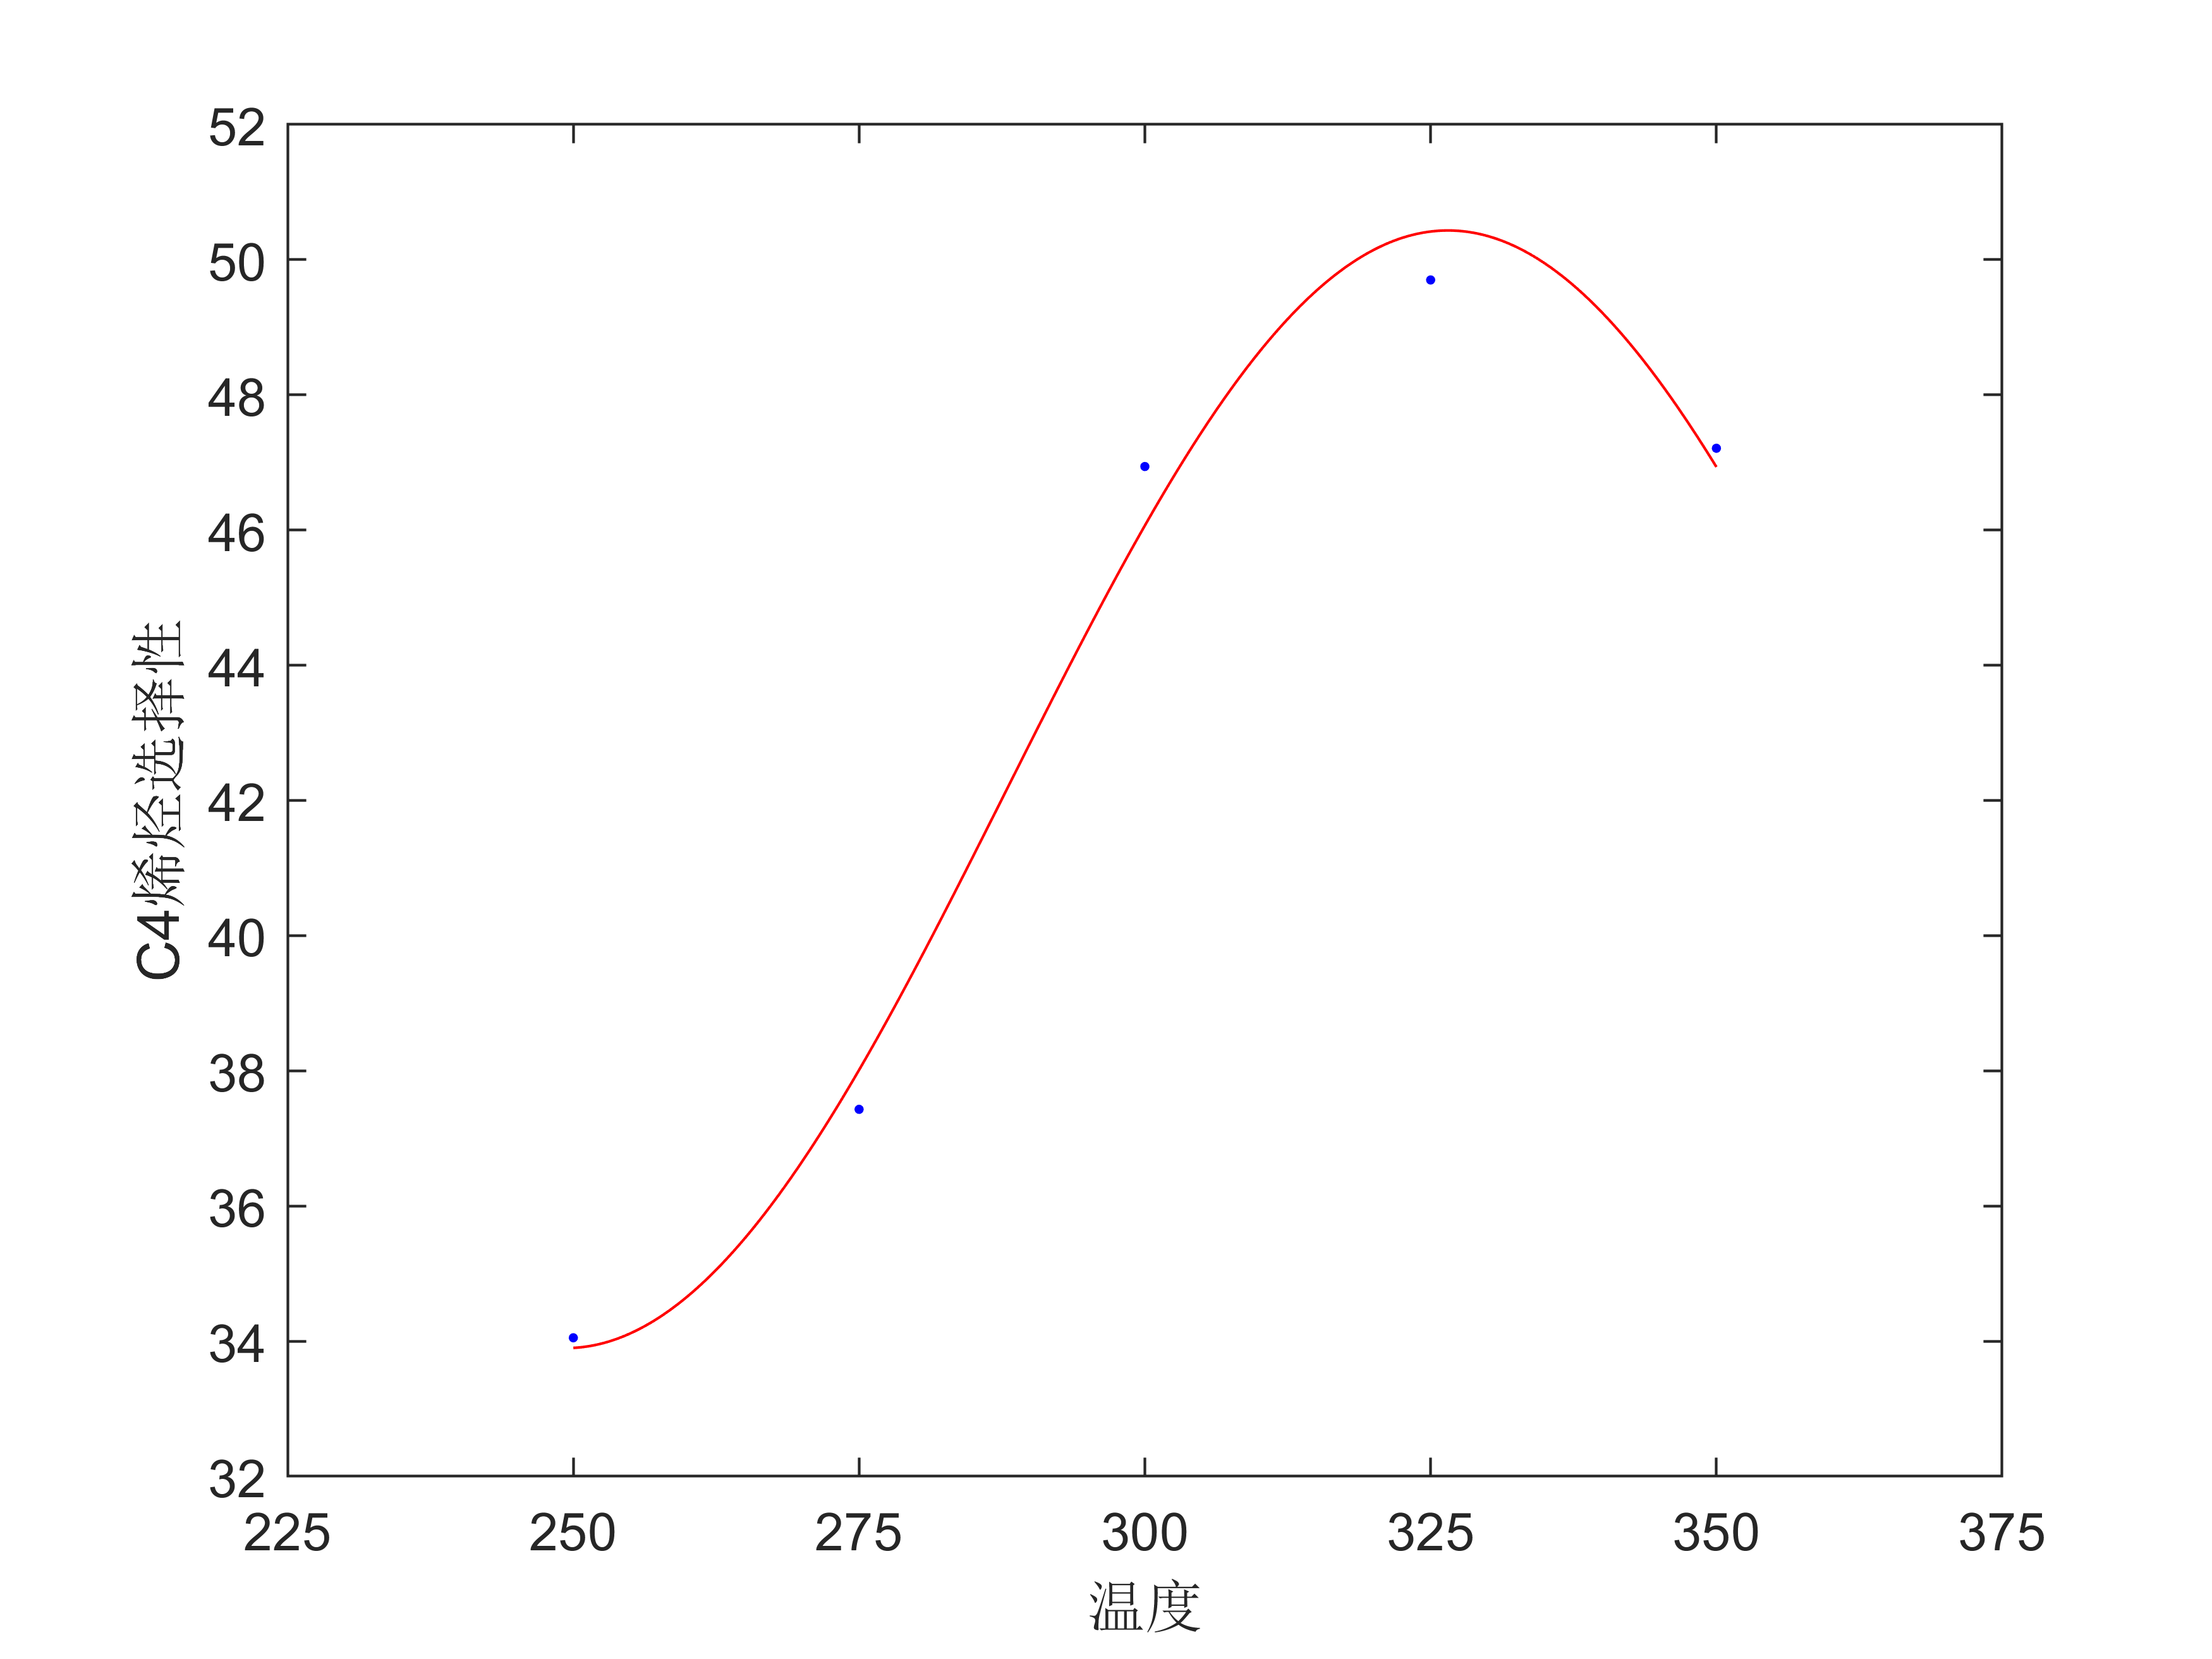
\includegraphics[width=9cm]{A1temp-c4.png}
\caption{\centering $A_1$催化剂中C$_4$烯烃选择性关于温度的拟合函数}
\end{minipage}
\begin{minipage}[t]{0.48\textwidth}
\centering
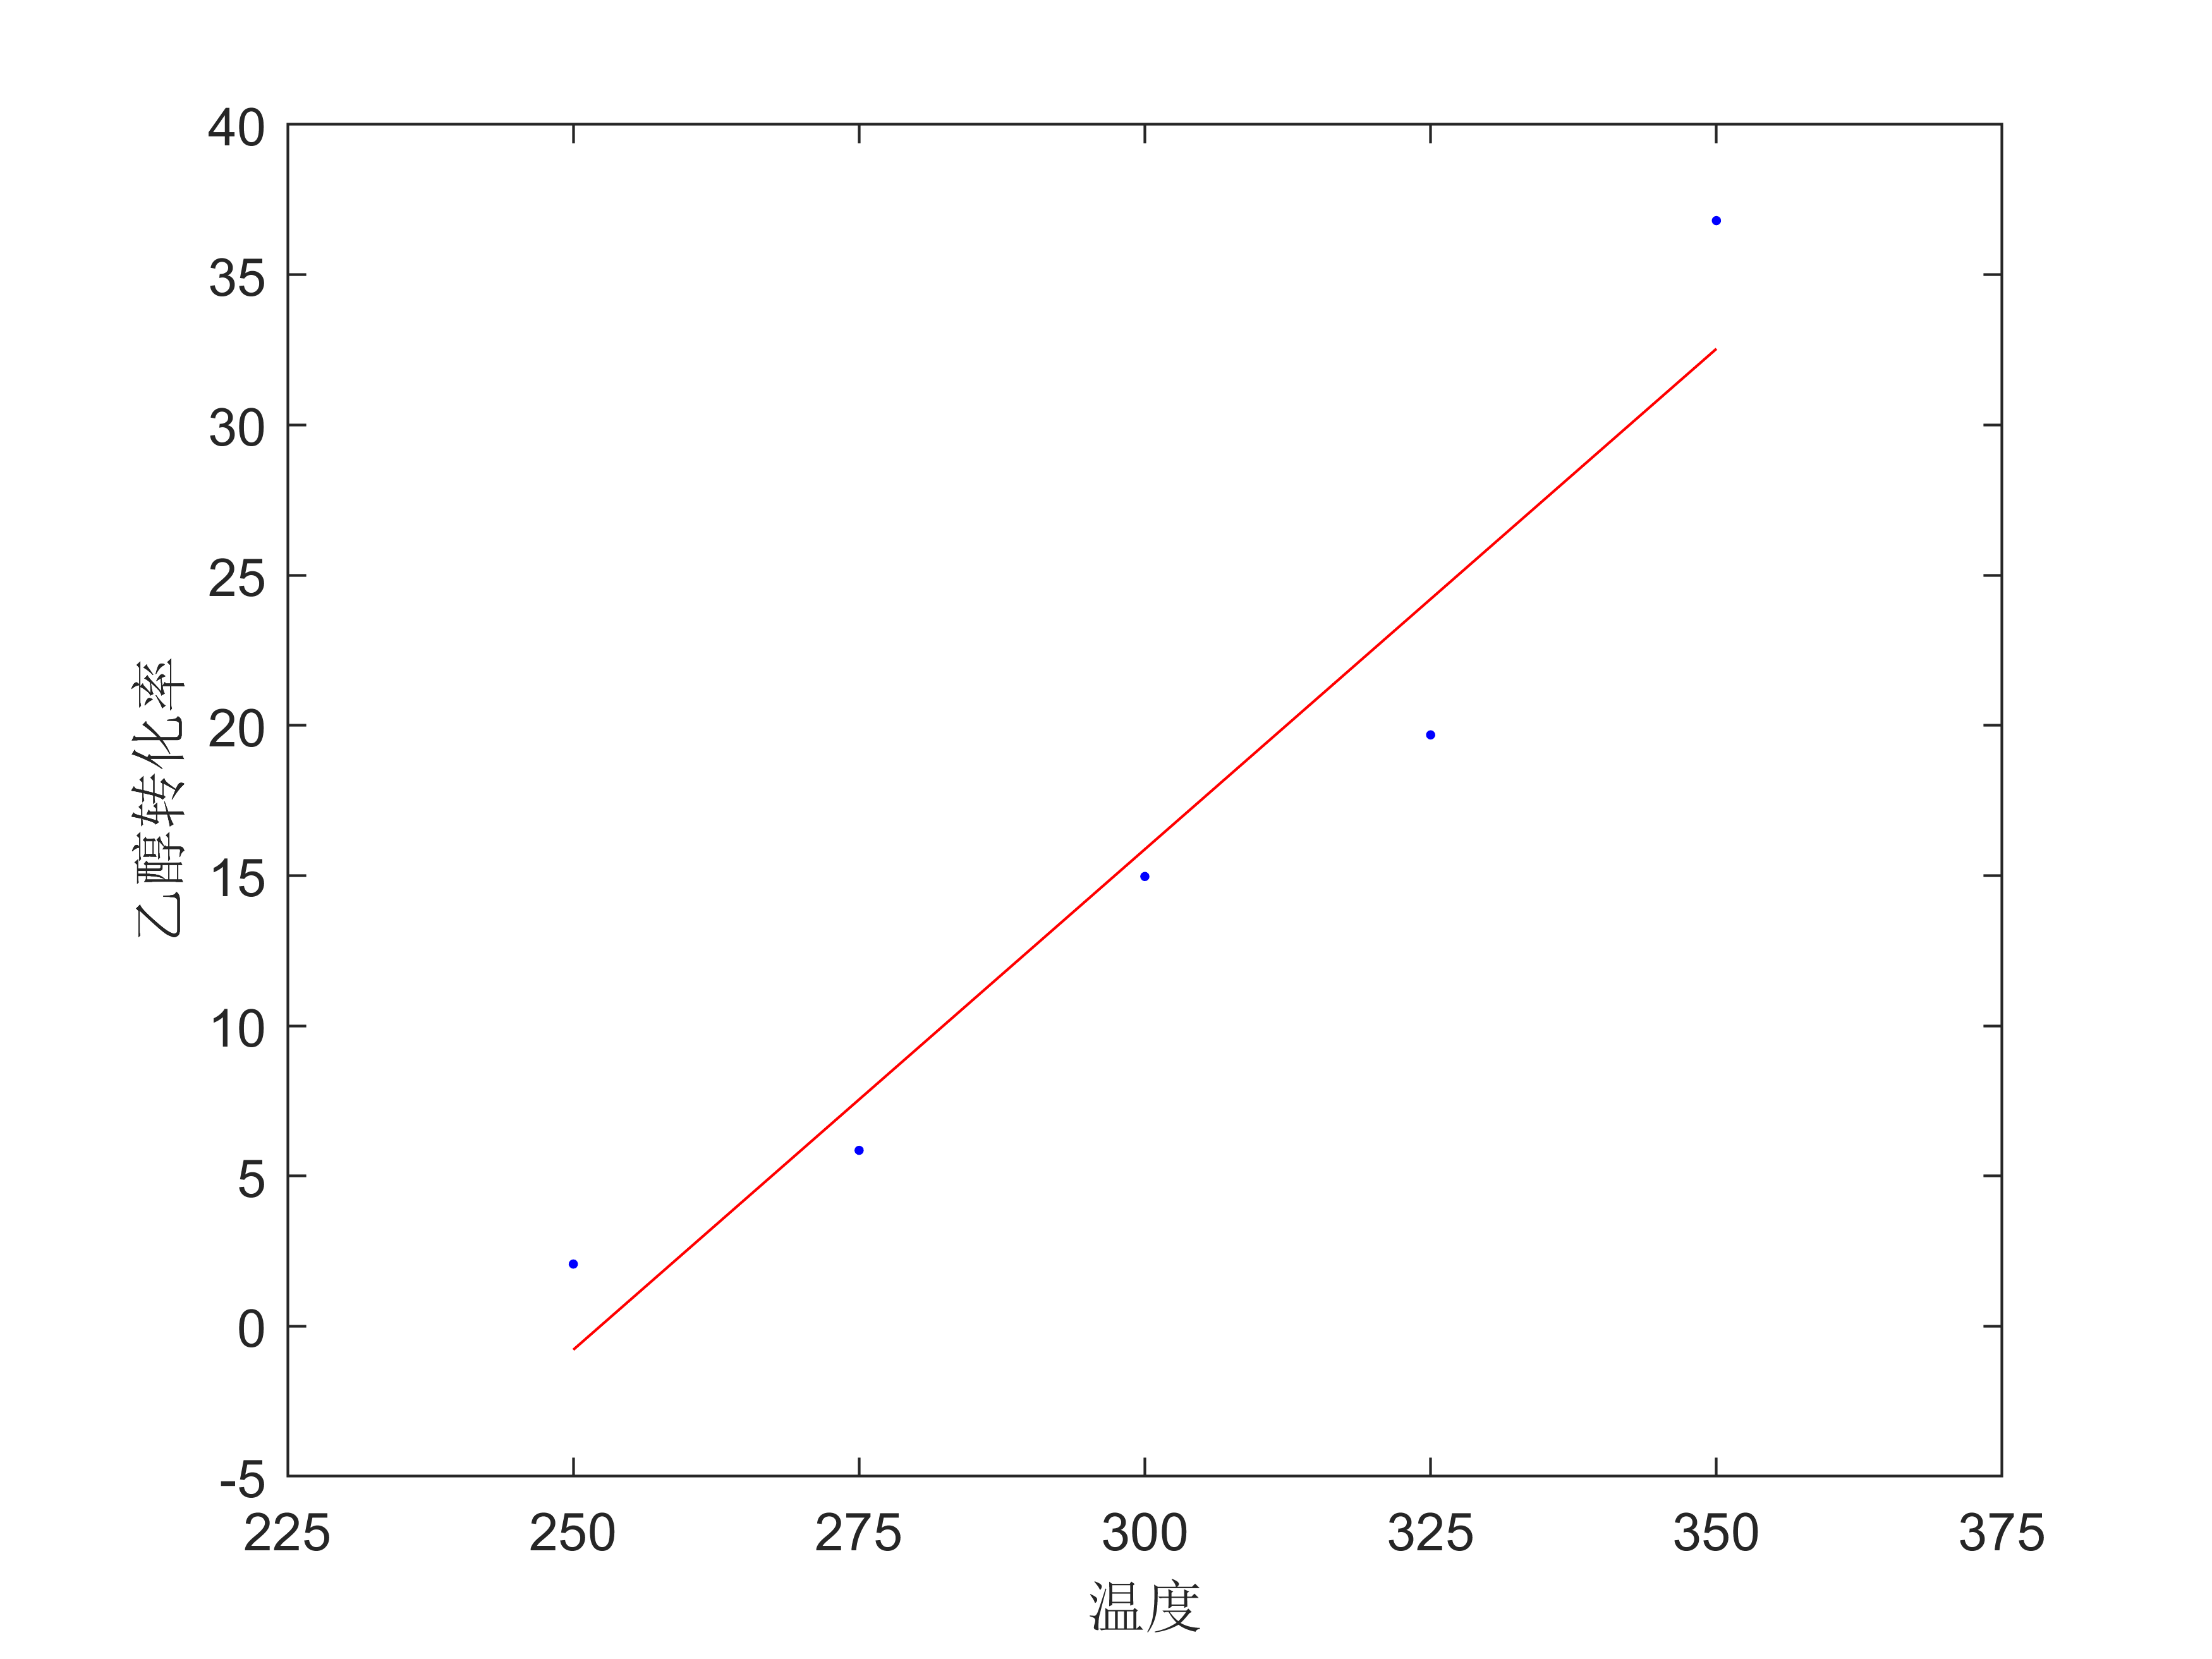
\includegraphics[width=9cm]{A1temp-乙醇.png}
\caption{\centering $A_1$催化剂中乙醇转化率关于温度的\\拟合函数}
\end{minipage}
\end{figure}
\input{图片插入.txt}

\end{document}